% ============================================================
%  CLIME: Cross-Modal Injection via Learned Market Encoding
%  深度学习基础课程大作业 — 最终报告
% ============================================================
\documentclass[12pt,a4paper]{ctexart}

% ---- Packages ----
\usepackage[top=2.5cm, bottom=2.5cm, left=2.8cm, right=2.8cm]{geometry}
\usepackage{amsmath,amssymb,amsfonts}
\usepackage{graphicx}
\usepackage{booktabs}
\usepackage{longtable}
\usepackage{multirow}
\usepackage{array}
\usepackage{caption}
\usepackage{subcaption}
\usepackage{hyperref}
\usepackage{enumitem}
\usepackage{float}
\usepackage{xcolor}
\usepackage{url}
\hypersetup{hidelinks}

% Force figures to stay in their section
\numberwithin{figure}{section}
\numberwithin{table}{section}

% ---- Metadata ----
\title{\textbf{CLIME: 跨模态市场信息注入的股票排序模型}\thanks{组员分工：费维瀚负责项目整体推进、模型设计与实现、实验分析、模拟交易复盘和报告主体撰写；赵瀚焜、寇之洲参与项目讨论、报告审阅，并对实验呈现和最终表述提供修改建议。} \\
       \large 深度学习基础课程大作业}
\author{费维瀚（PB24000347）\\
赵瀚焜（PB24000385）\quad 寇之洲（PB24000354）}
\date{\today}

\begin{document}

\maketitle

% ============================================================
% ============================================================
%  Abstract
% ============================================================
\begin{abstract}
\noindent
本项目研究的是A股日频选股中的\textbf{横截面排序信号}：在每日约4000--5000只可交易股票中，模型需要判断哪些股票相对更值得进入top-20组合。我们不把任务简化为单股次日收益的精确回归，也不声称构建了完整的真实交易系统；本文的核心评估对象是模型在holdout集上的排序能力和选股信号质量，交易成本、滑点、换手约束等执行层因素作为后续交易策略模块处理。基于这一设定，本文提出\textbf{CLIME}（Cross-Modal Injection via Learned Market Encoding），一种面向股票排序的Transformer架构。模型通过两阶段训练先学习pairwise排序先验，再使用方向感知回归损失进行精调；同时，ScaledGatedEncoder将同业动态（peer dynamics）和市场上下文以受控加法方式注入Backbone表征，使市场信息作为增量修正而非直接覆盖个股判断。

在holdout测试集（2025年12月至2026年5月，100个交易日）上，CLIME取得\textbf{+137.15\%累计收益}和\textbf{+123.14\%超额收益}（Sharpe 6.94），比最强基线Ridge（+91.65\%超额）高出约31个百分点，并在全部6个持有月保持正超额。消融实验表明，Stage~1预训练、BCE课程预热、Directional Regression Loss和ScaledGatedEncoder均对性能有明显贡献，其中训练策略组件的影响大于架构组件。除收益对比外，本文还通过Jacobian/SVD、线性探针、特征重要性和极端行情切片分析模型内部行为，验证模型确实利用了横截面排名、基本面和同业上下文等信号，而不是仅依赖单股历史趋势。

最后，本文记录了一次同花顺模拟交易作为端到端压力测试。该模拟最终收益为$-19.40\%$，显著弱于离线结果；但逐日调仓记录显示，主要问题来自日频信号与盘中人工执行之间的协议差异，包括非固定买入时点、先卖后买的资金释放约束、弱势市场下的人工择时压力和后期仓位集中。因此，该结果被解释为\textbf{执行层异常案例}，而不是CLIME离线排序能力的直接否定。它进一步说明，alpha predictor、risk/scoring、portfolio selection和execution必须作为不同模块分别建模。

\end{abstract}

% ============================================================
% ============================================================
%  1. Introduction
% ============================================================
\section{Introduction}
\label{sec:intro}

本文以课程大作业中的A股日频选股任务为背景，并采用research-style technical report的组织方式。为了让报告保持可读性，本文始终围绕一个核心问题展开：\textbf{能否学习一个稳定的横截面选股信号，使模型每天把更值得买入的股票排到前面？} 在全市场约5000只股票中每日选出top-20持仓，本质上是一个横截面排序问题：投资决策主要取决于股票之间的相对顺序，而非对单只股票次日收益的精确回归。

需要强调的是，本文研究的是\textbf{信号层}而非完整\textbf{交易执行层}。我们的离线评估协议使用top-20等权日调仓来横向比较不同模型的排序能力；该协议有利于检验模型是否能在holdout集上稳定选出相对更优的股票，但并未完整建模手续费、滑点、涨跌停成交约束、换手率控制和多日持有优化。因此，本文报告的离线收益指标应理解为受控协议下的选股信号表现，而不是可直接落地的真实净收益策略。为了检验从模型信号到真实操作之间的差距，本文还记录了一次同花顺模拟交易；该模拟结果较差，但它衡量的是“日频alpha信号+人工盘中执行”的端到端过程，而不是CLIME纯排序信号本身。

我们的核心诊断有两点。第一，股票预测的训练目标需要更贴近最终的排序决策。一方面，学习排序和偏好学习中的经验表明，pairwise supervision适合学习相对判断~\cite{joachims2002optimizing,burges2005learning,rendle2009bpr,christiano2017deep,ouyang2022training}；另一方面，单纯回归损失会对所有数值误差施加近似对称惩罚，却无法区分“方向错误”和“幅度略有偏差”这两类在选股中影响完全不同的错误。第二，只看单只股票自己的历史序列通常不够：A股中的行业联动、风格轮动和市场状态会同时影响一批股票。若模型完全看不到同业和市场上下文，其上限会受到明显限制。

因此，本文最重要的设计不是简单堆叠更大的Transformer，而是引入\textbf{peer-aware market context}：对每只股票构造top-10相似同业的动态统计量，并与市场上下文一起注入模型。市场信息的注入也需要谨慎处理：简单拼接市场指数或同业信息可能把噪声直接送入Backbone，而不是形成对个股判断的有约束修正。CLIME中的ScaledGatedEncoder正是为了解决这一点：它只学习一个受门控和幅度约束的表征偏移，让peer dynamics作为增量修正进入模型。

基于这些观察，我们提出\textbf{CLIME}（Cross-Modal Injection via Learned Market Encoding），一种面向股票排序的Transformer架构。CLIME包含三项关键设计：(1)~Stage~1使用pairwise ranking loss预训练Backbone，先学习通用排序先验；(2)~Stage~2通过BCE方向预热和Directional Regression Loss逐步过渡到次日收益预测；(3)~ScaledGatedEncoder将同业动态和市场上下文以受控加法方式注入表征空间，使市场信息作为增量修正而非直接覆盖个股判断。主实验均使用纯alpha分数（$\lambda=0$）评估CLIME本身的排序能力；风险过滤器仅作为模拟交易中的工程补充。

这种拆分也决定了本文对模拟交易结果的解释方式。若离线排序模型表现较好，但盘中模拟交易收益较差，不能简单得出“模型没有学到信号”的结论。真实收益还受到买入时点、卖出顺序、资金释放、仓位集中、人工择时和市场日内路径的影响。换言之，最终交易收益可以被视为alpha信号、组合构造、执行价格和人工干预的叠加结果。第~\ref{sec:trading}节将展示一个失败的模拟交易案例，并将其作为执行层缺口分析，而不是作为CLIME离线排序能力的主要评价指标。

在holdout测试集（2025年12月至2026年5月，共100个交易日）上，CLIME取得\textbf{累计收益+137.15\%、超额收益+123.14\%}（Sharpe 6.94），相对最强基线Ridge（+91.65\%超额）高出约31个百分点。消融实验显示，Stage~1预训练、BCE课程预热、Directional Regression Loss和ScaledGatedEncoder的移除都会造成明显退化；内部分析进一步表明，模型主要依赖横截面排名、基本面等信号，并形成了紧凑的主导排序方向。

本文的贡献可以概括为四点：第一，将A股日频选股明确建模为top-K排序任务，并清楚区分选股信号评估与真实交易执行；第二，设计了peer dynamics驱动的受控市场信息注入机制，而不是只依赖单股历史序列；第三，通过基线对比、消融实验、Jacobian/SVD、线性探针、特征重要性和极端行情切片，同时评估模型收益、组件贡献和可解释性；第四，结合模拟交易记录分析离线alpha信号到真实执行之间的断层，说明一个表现较好的predictor仍需要独立的portfolio construction和execution模块才能成为完整量化系统。

% ============================================================
% ============================================================
%  2. Methodology
% ============================================================
\section{Methodology}
\label{sec:method}

\subsection{Problem Formulation}

对于交易日$t$，给定$N_t$只股票的历史特征序列$\mathbf{x}_i^{(t)} \in \mathbb{R}^{L \times F}$（$L=40$个交易日，$F=67$维特征），以及每只股票的同业动态特征$\mathbf{p}_i^{(t)} \in \mathbb{R}^{24}$，模型输出一个标量alpha分数$s_i^{(t)}$。该分数不是最终交易指令，而是用于横截面排序的选股信号。每日评估时，我们选取分数最高的$K=20$只股票构建等权组合，持有一个交易日后卖出，以此衡量模型是否能把次日相对收益更高的股票排在前面。预测标签为次日收益率$r_i^{(t)} = \frac{\text{close}_{i}^{(t+1)} - \text{close}_{i}^{(t)}}{\text{close}_{i}^{(t)}}$。股票池为除ST股和北交所外的全部A股。

这种表述刻意将系统拆成两层：\textbf{预测/排序层}负责产生alpha分数，\textbf{交易策略层}负责处理交易成本、滑点、换手率、风险预算和实际成交约束。本文主要研究前者；后者只在第\ref{sec:risk}节和第\ref{sec:trading}节作为工程扩展讨论。

\subsection{Feature Design}

\subsubsection{Stock Features}

我们使用67维个股特征，覆盖收益、量价、技术指标、基本面、资金流向、市场指数、市场宽度、横截面相对排名和位置编码等类别。特征设计参考Kakushadze的101 Formulaic Alphas~\cite{kakushadze2016alphas}，目标是系统性覆盖常见量化因子类型，而非手工筛选少数单一因子。所有特征逐日进行横截面标准化，仅使用当日及历史数据；完整特征列表见附录\ref{sec:appendix_features}。

\subsubsection{Peer Dynamics}

Peer Dynamics为每只股票提供同业群体的统计画像，这是本文区别于普通单股序列模型的关键输入。直觉上，某只股票的短期表现往往不只由自身历史决定，还受到同业共同上涨/下跌、行业轮动、风格切换和相对强弱变化影响。因此，我们基于行业、业务描述、地区、企业类型和历史收益相关性选取top-10相似股票，并聚合同业收益、成交活跃度、技术指标、基本面和个股相对偏差等24维特征。

相比直接输入全市场所有股票，Peer Dynamics是一种低成本、可解释的局部市场上下文：模型看到的是“与当前股票最相关的一组股票正在发生什么”，而不是无结构的全市场噪声。相比只输入市场指数，它又保留了行业和同业层面的细粒度差异。相似度权重和聚合细节见附录\ref{sec:appendix_features}。

\subsection{Model Architecture}

模型整体架构如图\ref{fig:architecture}所示，采用双流设计：Backbone处理个股特征序列，ScaledGatedEncoder处理peer dynamics和市场上下文，两者在表征空间通过加法融合。这样的拆分使模型既能保留单股历史序列中的主信号，也能在必要时利用同业和市场状态修正判断。

\begin{figure}[H]
\centering
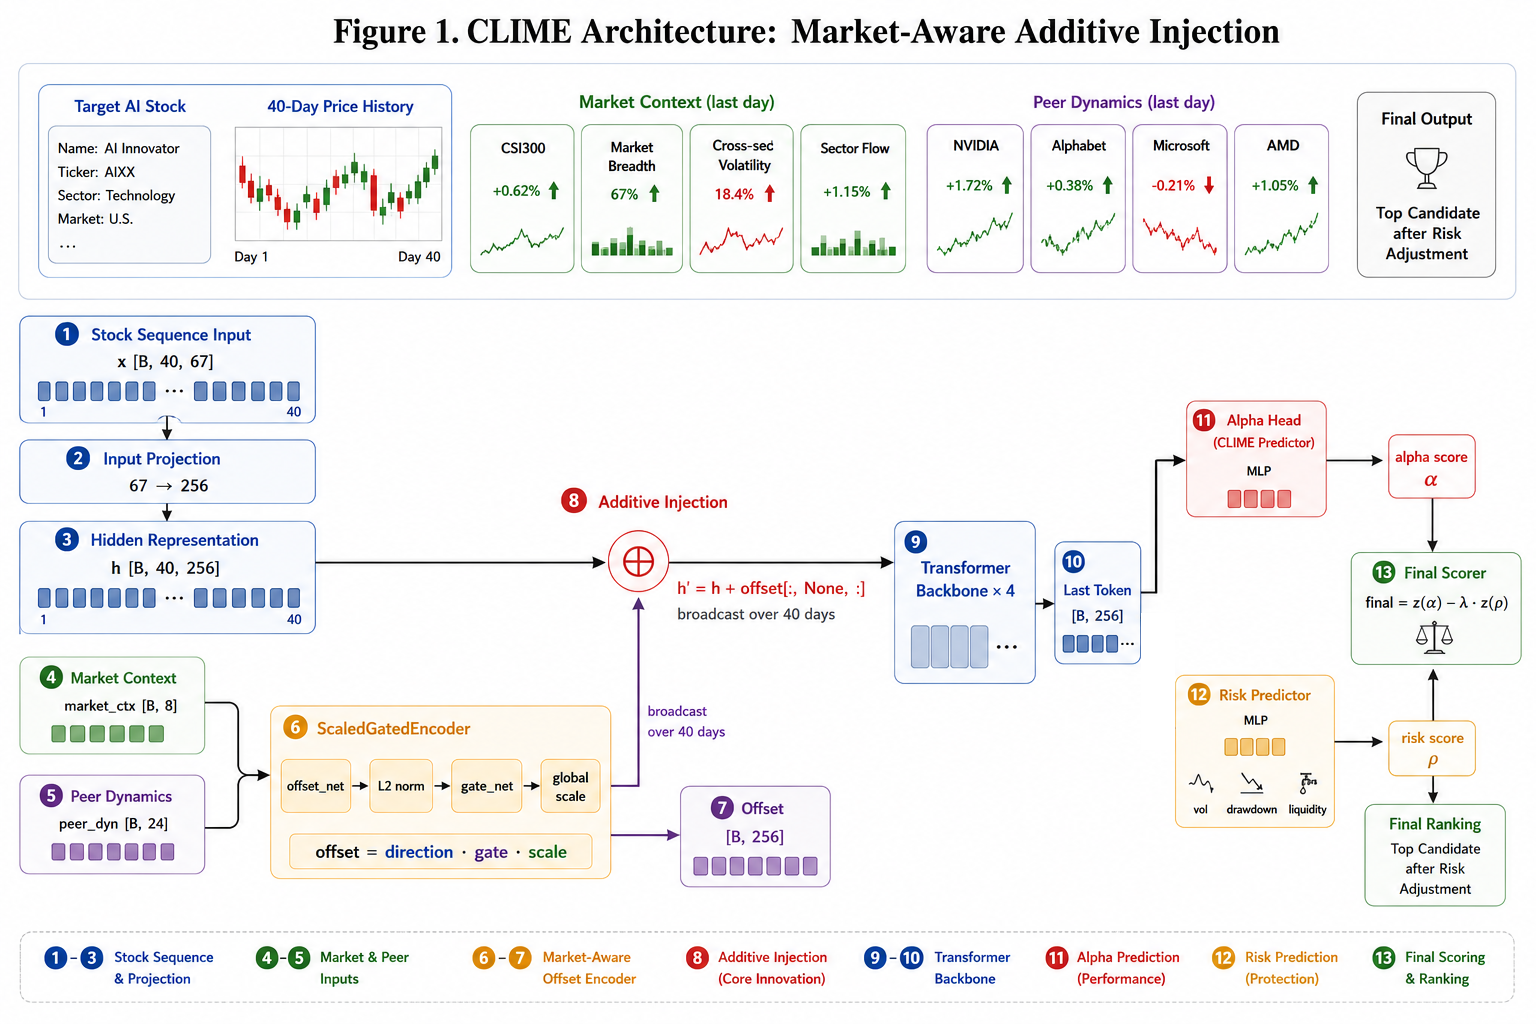
\includegraphics[width=\textwidth]{figures/architecture.png}
\caption{CLIME模型架构。左侧输入：个股特征序列$\mathbf{x} \in \mathbb{R}^{B\times40\times67}$和同业动态$\mathbf{p} \in \mathbb{R}^{B\times24}$。中下部：ScaledGatedEncoder将peer\_dyn与market\_ctx拼接，经offset\_net生成方向向量，由gate\_net选择性门控和全局scale约束后产生offset。中上部：Backbone通过input\_proj将$\mathbf{x}$映射到256维表征空间，与offset加法融合后经RoPE和4层Transformer处理。右侧：预测头输出标量分数。}
\label{fig:architecture}
\end{figure}

\subsubsection{Transformer Backbone}

Backbone为标准Transformer结构：input\_proj（$67 \to 256$）、旋转位置编码（RoPE）、4层TransformerBlock（Multi-Head Attention, 8 heads, $d=256$；Feed-Forward hidden=1024；Pre-LN），最后通过last-token extraction（$\mathbf{h}[:, -1, :]$）获取序列表示。Backbone参数量约2.3M，采用标准的Transformer配置，架构细节在此不做赘述。

\subsubsection{ScaledGatedEncoder}

ScaledGatedEncoder是整个架构的核心组件，也是peer dynamics进入模型的主要通道。它的目标不是重新生成一个完整预测，而是在Backbone已经形成的个股表示上学习一个有约束的市场修正项。该模块由三个子模块构成：

\textbf{offset\_net}将peer\_dyn（24维）与market\_ctx（8维）拼接后映射为原始偏移向量$\hat{\mathbf{u}} \in \mathbb{R}^{256}$，并进行L2归一化：$\mathbf{u} = \hat{\mathbf{u}} / \|\hat{\mathbf{u}}\|$。这一设计使encoder主要控制修正方向，而不直接控制修正幅度。

\textbf{gate\_net}根据market\_ctx输出门控值$g \in [0, 1]$，为每只股票独立控制市场修正强度。该模块实现\textbf{选择性注入}：不同股票可以接收不同程度的市场上下文。

\textbf{logit\_scale}是一个全局可学习标量，经tanh约束后控制offset幅度。最终offset合成为：
\begin{equation}
\text{offset} = g \cdot \tanh(s) \cdot \frac{\hat{\mathbf{u}}}{\|\hat{\mathbf{u}}\|} \cdot \sqrt{256}
\end{equation}

\subsubsection{加法注入与设计原则}

市场信息通过加法注入Backbone的表征空间：
\begin{equation}
\mathbf{h}' = \mathbf{h} + \text{offset} \quad (\text{offset广播到所有40个时间步})
\end{equation}

这一加法设计与FiLM式乘性调制（$\gamma \odot \mathbf{h} + \beta$）形成对比。乘性调制可能直接改变Backbone已学到的表征，而加法注入保留原始判断，只学习增量修正。这一思想与Adapter~\cite{houlsby2019adapter}和LoRA~\cite{hu2022lora}等加性微调方法相近。

三个约束共同限制市场调制的影响范围：unit-norm控制方向，gate控制个股层面的注入强度，tanh约束全局幅度。因此Backbone仍是主信号，市场信息只做受控修正。

\subsection{Training Pipeline}

整体训练流程如图\ref{fig:training}所示，分为两个阶段。

\begin{figure}[H]
\centering
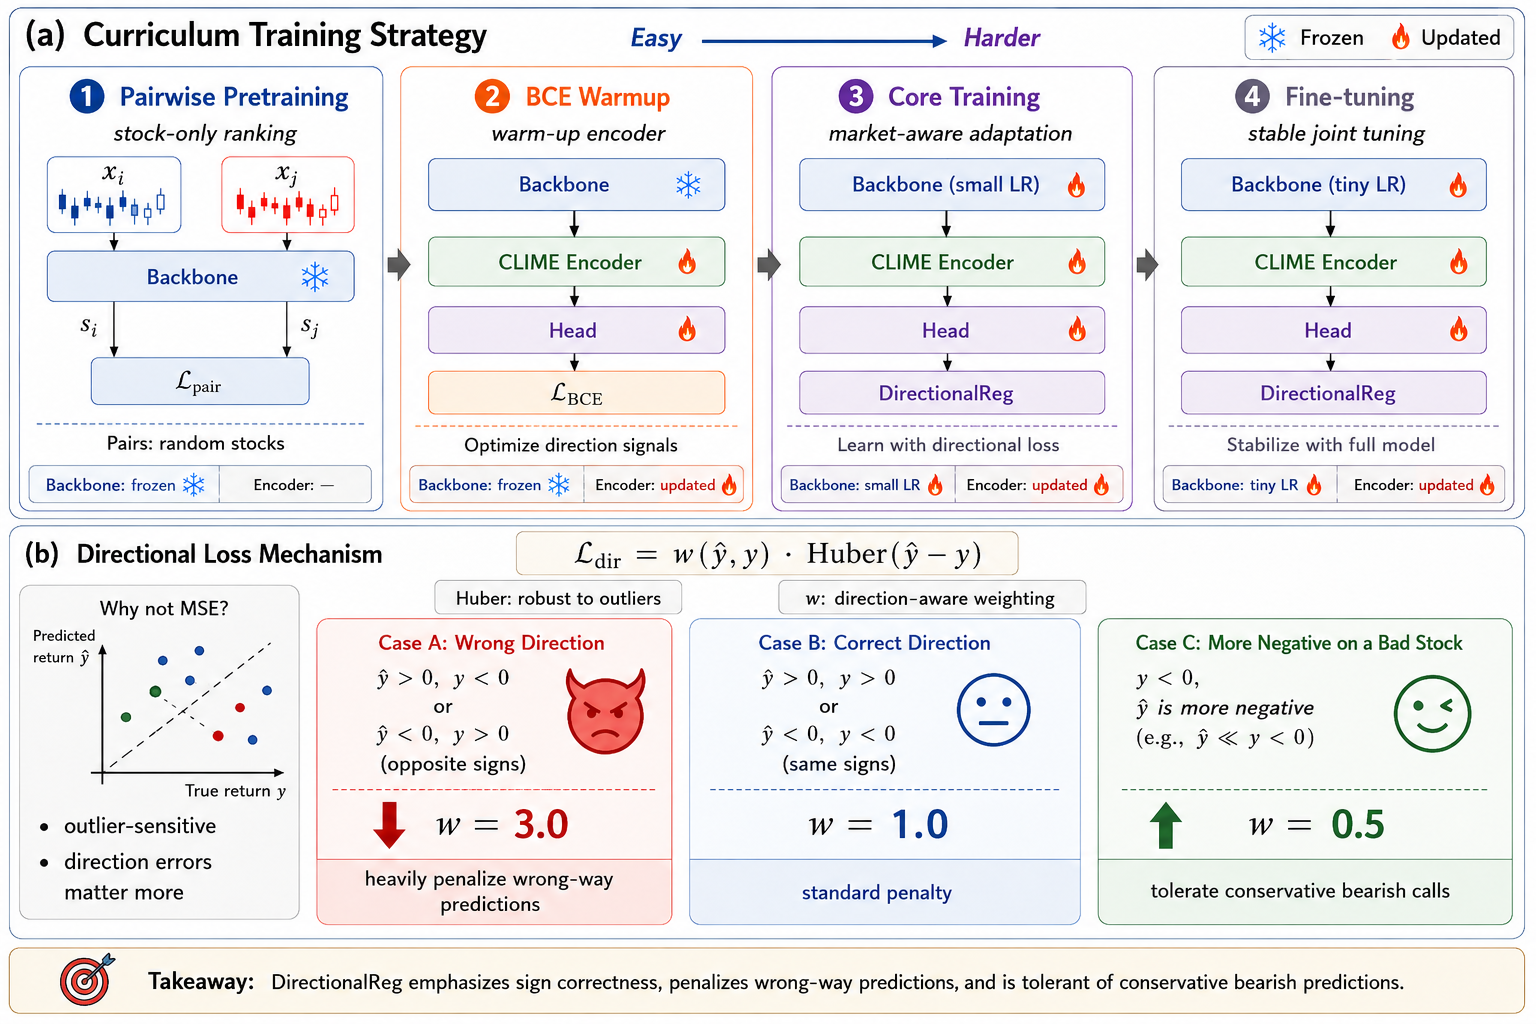
\includegraphics[width=\textwidth]{figures/training.png}
\caption{两阶段训练流程。Stage~1：使用Pairwise Ranking Loss预训练纯Backbone。Stage~2：加载Stage~1权重，冻结Backbone进行3个epoch的BCE方向预热，随后解冻Backbone以极小学习率（encoder的1/50）进行DirectionalReg核心训练，最后以更低学习率精调。}
\label{fig:training}
\end{figure}

\subsubsection{Stage 1: Backbone Pretraining}

Stage~1的目标是让Backbone学会从67维量价特征中提取通用模式，暂不涉及市场信息。采用\textbf{PairDataset}构造训练数据：每日对股票按收益率排序，分别从top-10\%和bottom-10\%中采样并随机配对，生成约5000个pair样本。配对约束要求pair间的收益率差大于margin=0.002，确保pair具有足够区分度。

采用\textbf{Pairwise Ranking Loss}：
\begin{equation}
\mathcal{L}_{\text{pair}} = \log(1 + \exp(-y \cdot (s_i - s_j)))
\end{equation}
其中$y = +1$表示股票$i$的收益率高于股票$j$。该损失直接优化相对排序——训练初期模型无需精确预测“好多少”，只需学会判断“谁更好”。这是一个比精确值回归更简单的学习任务，为后续课程学习奠定了基础。Early Stopping以验证集上的Top-20 Excess Return为唯一指标。

\subsubsection{Stage 2: Three-Phase Curriculum Training}

Stage~2加载Stage~1预训练的Backbone权重，通过三阶段课程训练逐步引入市场调制能力和精细预测能力。各阶段配置见表\ref{tab:stage2_phases}。

\begin{table}[H]
\centering
\caption{Stage 2 三阶段课程训练配置}
\label{tab:stage2_phases}
\begin{tabular}{@{}cclccc@{}}
\toprule
Phase & Epochs & Loss & Backbone & Encoder \& Head \\
\midrule
1 (BCE Warmup)  & 1--3  & BCEWithLogitsLoss  & \textbf{Frozen} & $10^{-3}$ \\
2 (Core)        & 4--15 & DirectionalReg Loss & $10^{-5}$       & $5\times10^{-4}$ \\
3 (Fine-tune)   & 16--25& DirectionalReg Loss & $10^{-6}$       & $5\times10^{-4}$ / $10^{-5}$ (head) \\
\bottomrule
\end{tabular}
\end{table}

\textbf{Phase 1（BCE预热）}：冻结Backbone，仅用涨跌方向分类任务训练随机初始化的encoder和head，避免回归损失的早期噪声破坏预训练表示。

\textbf{Phase 2（核心训练）}：切换到Directional Regression Loss，解冻Backbone并以远小于encoder的学习率微调，使市场编码器逐步适配已有排序表征。

\textbf{Phase 3（精调）}：所有学习率降低，系统在最优解附近精细化收敛。

完整训练超参数见附录\ref{sec:appendix_hyperparams}。

\subsubsection{Directional Regression Loss}

Directional Regression Loss是本工作的核心损失函数设计，旨在桥接回归的精确性与排序的感知能力。基础层使用Huber Loss（$\delta=0.01$）以对抗极端收益值（涨停/跌停）：
\begin{equation}
H_{0.01}(e) = \begin{cases}
0.5 e^2 & \text{if } |e| \leq 0.01 \\
0.01(|e| - 0.005) & \text{if } |e| > 0.01
\end{cases}
\end{equation}

上层乘以方向感知的非对称权重：
\begin{equation}
w(\hat{r}, r) = \begin{cases}
3.0 & \text{if } \operatorname{sign}(\hat{r}) \neq \operatorname{sign}(r) \quad \text{【方向错误】}\\
0.5 & \text{if } \operatorname{sign}(\hat{r}) = \operatorname{sign}(r) < 0 \text{ and } \hat{r} < r \quad \text{【保守悲观】}\\
1.0 & \text{otherwise} \quad \text{【正常】}
\end{cases}
\end{equation}
\begin{equation}
\mathcal{L} = \frac{1}{N}\sum_{i=1}^{N} w(\hat{r}_i, r_i) \cdot H_{0.01}(\hat{r}_i - r_i)
\end{equation}

三个权重的设计逻辑与选股场景精确对应：
\begin{itemize}[leftmargin=*, itemsep=2pt]
    \item \textbf{方向错误}（$\times 3$）：预测方向与实际收益方向相反，对top-20排序影响最大。
    \item \textbf{保守悲观}（$\times 0.5$）：方向正确但预测偏低，该股票通常不会进入top-20，因此降低其梯度权重。
    \item \textbf{正常}（$\times 1$）：方向正确且不满足保守悲观条件，标准Huber惩罚。
\end{itemize}

与纯排序损失（pairwise/listwise）相比，DirectionalReg保留了收益幅度信息；与纯回归损失（MSE）相比，DirectionalReg将优化目标重新对齐到了选股的真实需求——\textbf{只需要相对顺序正确，不需要精确预测每一个基点}。后续消融实验（RQ2）将量化验证这一设计的贡献。

\subsection{Risk-Adjusted Scoring}
\label{sec:risk}

CLIME模型输出alpha分数后，在实际交易中可以叠加一个规则驱动的风险过滤器。该过滤器基于过去20日波动率、回撤、振幅和流动性风险构造综合风险分数，最终交易决策分数为：

\begin{equation}
\text{final}_i^{(t)} = z(\alpha_i^{(t)}) - \lambda \cdot z(\text{risk}_i^{(t)})
\end{equation}

并在alpha分数前10\%的候选池内进行风险调整排序。该模块无可学习参数，实验部分的所有评估均使用纯alpha分数（$\lambda = 0$）；同花顺模拟交易中使用$\lambda=0.3$作为更保守的执行配置。完整配置见附录\ref{sec:appendix_risk}。

% ============================================================
% ============================================================
%  3. Experiments
% ============================================================
\section{Experiments}
\label{sec:experiment}

为系统评估CLIME的有效性，我们围绕三个核心研究问题组织实验：
\begin{itemize}[leftmargin=*, itemsep=4pt]
    \item \textbf{RQ1（性能对比与稳定性）}：CLIME在holdout测试集上是否显著优于强基线模型？其优势是否在不同的时间跨度和市场环境中保持稳健？
    \item \textbf{RQ2（消融分析）}：两阶段课程训练、Directional Regression Loss、BCE方向预热、ScaledGatedEncoder——各个设计组件对最终性能的贡献有多大？
    \item \textbf{RQ3（内部分析）}：模型学到了什么？ScaledGatedEncoder是否真正实现了差异化的市场信息注入？
\end{itemize}

所有实验均以模型在holdout测试集上的\textbf{受控top-20选股表现}作为最终评价标准。这里的“投资表现”用于横向比较模型排序信号的强弱，而非声称已经覆盖真实交易执行中的全部约束。除非特殊说明，我们以超额收益、Sharpe、最大回撤和胜率作为主要判据，同时在消融实验（RQ2）和内部分析（RQ3）中辅以RankIC（Rank Information Coefficient）作为统计诊断工具。

\textbf{重要说明}：本章所有实验均使用\textbf{纯alpha分数}（即CLIME模型的原始输出，不经风险调整，$\lambda = 0$），以隔离模型本身的排序能力。第\ref{sec:risk}节描述的风险过滤器仅在同花顺模拟交易（第\ref{sec:trading}节）中启用。这种解耦设计确保实验评估的是CLIME的选股信号本身，而非风险过滤器、换手控制或交易执行规则的附加效果。

\subsection{Dataset and Preprocessing}
\label{sec:dataset}

\subsubsection{Data Source and Feature Computation}

原始数据来源于聚宽（JoinQuant）量化平台，涵盖全部A股（剔除ST股和北交所股票后约4000--5000只）的日频交易数据、基本面指标、资金流向数据和市场指数。数据时间范围为2015年1月至2026年5月。基于原始数据，我们计算67维量价特征（详见第\ref{sec:method}节及附录\ref{sec:appendix_features}），涵盖收益类、量价类、技术指标、基本面、资金流向、市场指数、市场宽度和横截面相对排名8个类别。

\subsubsection{Data Hygiene and Leakage Prevention}

金融数据容易因时间自相关和预处理方式引入\textbf{前瞻偏差}（look-ahead bias）。为保证评估可信，本文的数据管线遵循三条原则：

\begin{enumerate}[leftmargin=*, itemsep=2pt]
    \item \textbf{时点对齐}：交易日$t$的所有特征只使用$\le t$的信息，标签为$t+1$日收益。
    \item \textbf{逐日横截面处理}：缺失值填充、Winsorize和z-score均在同一交易日内独立完成，不跨日期拟合统计量。
    \item \textbf{时间切分}：训练、验证、holdout严格按日期划分且互不重叠；holdout不参与任何模型选择。
\end{enumerate}

此外，我们保留2026年5月12日至5月26日的9个交易日作为纯未来验证集，不参与训练、验证、holdout评估或任何决策。更详细的数据卫生检查见附录\ref{sec:appendix_eval_details}。

\subsubsection{Feature Preprocessing}

特征级预处理逐日执行：

\begin{enumerate}[leftmargin=*, itemsep=2pt]
    \item \textbf{缺失值填充}：以当日横截面中位数填充（逐日、逐特征独立处理，不使用跨期信息）。
    \item \textbf{极端值处理}：以当日横截面的1\%和99\%分位数进行Winsorize处理（逐日、逐特征独立计算，不跨日期拟合阈值）。
    \item \textbf{横截面z-score标准化}：如上所述，每日独立标准化，仅使用当日横截面均值和标准差。
\end{enumerate}

\subsubsection{Train / Validation / Holdout Split}

数据集按时间顺序划分为三个互不重叠的部分，如表\ref{tab:data_split}所示。训练集以step=10稀疏采样，验证集和测试集以step=1全密度评估。

\begin{table}[H]
\centering
\caption{数据集划分。所有划分严格按时间排序，互不重叠。}
\label{tab:data_split}
\begin{tabular}{@{}ccccc@{}}
\toprule
Split & Date Range & Trading Days & Step & Purpose \\
\midrule
Train (train\_v5)  & 2016-01-04 -- 2025-09-17 & $\sim$1700 & 10 & Model training \\
Validation (val\_v5) & 2025-09-18 -- 2025-12-04 & 50 & 1 & Hyperparameter selection \\
Holdout (holdout\_v5) & 2025-12-05 -- 2026-05-11 & 100 & 1 & Final evaluation \\
\bottomrule
\end{tabular}
\end{table}

验证集用于Stage~1和Stage~2的早停与超参数选择；holdout测试集在全部训练完成后仅评估一次。

\subsubsection{Stock Universe}

股票池为全部A股剔除ST股和北交所股票；ST状态按当日可得信息过滤。

\subsection{Experimental Settings}
\label{sec:exp_settings}

\subsubsection{Evaluation Protocol and Metrics}

评估遵循统一的\textbf{Top-20等权日调仓}协议：

\begin{enumerate}[leftmargin=*, itemsep=2pt]
    \item 在每个交易日$t$收盘后，模型对股票池中所有$N_t$只股票输出预测分数$s_i^{(t)}$；
    \item 选取分数最高的$K=20$只股票，以等权（每只5\%）构建投资组合；
    \item 在交易日$t+1$以收盘价卖出，组合日收益率$r_{\text{port}}^{(t)} = \frac{1}{20}\sum_{i \in \text{top-}20} r_i^{(t)}$，其中$r_i^{(t)} = \text{close}_i^{(t+1)} / \text{close}_i^{(t)} - 1$；
    \item 每日重复上述流程，累计收益为日收益的复利累积。
\end{enumerate}

所有实验均\textbf{不设交易成本}（单边0\%），以聚焦于模型选股能力本身的比较。组合权重严格等权，不做任何权重优化。

\subsubsection{Scope and Differences from Real Trading}

我们的实验协议用于评估模型选股信号，因此有意做了若干简化假设：

\begin{itemize}[leftmargin=*, itemsep=2pt]
    \item 不扣除交易成本和滑点；
    \item 假设所有top-20股票均可按收盘价成交；
    \item 不显式建模涨跌停、流动性冲击和多日持有策略。
\end{itemize}

因此，本文收益应被解读为\textbf{统一评估协议下的信号收益}，而非可直接提取的策略净收益。这样的协议适合回答“哪个模型在同一holdout set上排序更好”，但不能替代真实交易策略评估。真实交易系统还需要在alpha分数之后加入组合构建、交易成本、换手率控制、流动性过滤和成交约束；这些属于交易策略层，而不是本文主要优化的预测层。交易层约束的详细讨论见附录\ref{sec:appendix_eval_details}。

核心指标均以holdout测试集上的top-20组合表现为准：

\begin{itemize}[leftmargin=*, itemsep=2pt]
    \item \textbf{累计收益（Cumulative Return）}：$\prod_{t=1}^{T} (1 + r_{\text{port}}^{(t)}) - 1$
    \item \textbf{超额收益（Excess Return）}：$\prod_{t=1}^{T} (1 + r_{\text{port}}^{(t)}) - \prod_{t=1}^{T} (1 + r_{\text{market}}^{(t)})$，其中$r_{\text{market}}^{(t)}$为当日全部A股（除ST和北交所）的等权平均收益率。该指标度量模型相对于"闭眼随机买"的超额回报。
    \item \textbf{Sharpe Ratio}：年化夏普比率，$\text{Sharpe} = \frac{\bar{r}_{\text{excess}}}{\sigma(r_{\text{excess}})} \times \sqrt{250}$，其中$\bar{r}_{\text{excess}}$为日均超额收益，$\sigma(r_{\text{excess}})$为超额收益的标准差。无风险利率假设为0。
    \item \textbf{最大回撤 / 日胜率 / 月胜率}：用于衡量收益路径的稳定性。
\end{itemize}

\subsubsection{Baselines}

我们选取5类基线模型，覆盖线性模型、树模型和深度时序模型：

\begin{itemize}[leftmargin=*, itemsep=4pt]
    \item \textbf{Ridge}：使用最后一日67维特征的强线性基线~\cite{poh2020learning}。
    \item \textbf{XGBoost / LightGBM}~\cite{xgboost,lightgbm}：使用最后一日67维特征的梯度提升树模型。
    \item \textbf{MLP}：4层全连接网络，使用最后一日67维特征。
    \item \textbf{GRU}：2层循环网络，使用40日特征序列。
\end{itemize}

所有基线使用相同训练、验证和holdout划分。树模型以MSE回归训练，MLP和GRU使用与CLIME一致的数据预处理流程。

\subsubsection{Hyperparameters and Implementation}

CLIME的训练分为两个阶段，关键超参数如表\ref{tab:hyperparams}所示；完整的超参数配置和硬件环境见附录\ref{sec:appendix_hyperparams}。

\begin{table}[H]
\centering
\caption{CLIME训练关键超参数}
\label{tab:hyperparams}
\begin{tabular}{@{}lcc@{}}
\toprule
Hyperparameter & Stage 1 & Stage 2 \\
\midrule
Optimizer & Adam & Adam \\
Learning Rate & $5\times10^{-4}$ & $10^{-5}$ (backbone) / $5\times10^{-4}$ (encoder) \\
LR Scheduler & CosineAnnealing (T=40) & CosineAnnealing (T=25) \\
Batch Size & 2048 & 256 \\
Max Epochs & 40 & 25 \\
Early Stopping Patience & 10 & 8 \\
Weight Decay & $10^{-5}$ & $10^{-5}$ \\
Gradient Clip & 1.0 & 1.0 \\
Loss Function & Pairwise Ranking & BCE / DirectionalReg \\
\bottomrule
\end{tabular}
\end{table}

模型使用PyTorch实现，在NVIDIA A100（80GB）GPU上训练。Stage~1约需2小时，Stage~2约需1.5小时。模型总参数量约2.8M（Backbone约2.3M，ScaledGatedEncoder约0.5M）。所有报告结果均可由公开代码复现；从随机初始化重新训练得到的模型在holdout集上的核心收益指标与本文使用的best checkpoint差异控制在约5\%以内，说明结果不是单次随机种子或checkpoint选择的偶然产物。

% ============================================================
%  RQ1: Performance Comparison
% ============================================================
\subsection{RQ1: Performance Comparison and Stability}
\label{sec:rq1}

\subsubsection{Comparison with Baselines}

表\ref{tab:rq1_main}展示了CLIME与5个基线模型在holdout测试集（100个交易日）上的对比。市场等权组合同期累计收益为+14.01\%。

\begin{table}[H]
\centering
\caption{RQ1：Holdout测试集（2025-12-05 -- 2026-05-11，100个交易日）上的性能对比。最优结果以\textbf{粗体}标出，次优结果以下划线标出。RankIC$^*$列同时报告验证集与holdout集的值（Val / Holdout），用于诊断统计信号强度与泛化差距。}
\label{tab:rq1_main}
\resizebox{\textwidth}{!}{%
\begin{tabular}{@{}lrrrrrrr@{}}
\toprule
Model & Cum. Return & Excess & Sharpe & MaxDD & Daily Win & Monthly Win & RankIC$^*$ \\
\midrule
MLP      & $-$17.17\% & $-$31.18\% & $-$2.05 & 28.95\% & 34.0\% & 1 / 6 & 0.061 / 0.022 \\
GRU      & +13.92\%   & $-$0.09\%  & 0.02    & 12.48\% & 43.0\% & 3 / 6 & 0.070 / 0.047 \\
XGBoost  & +93.21\%   & +79.20\%   & 3.45    & 12.70\% & 57.0\% & 6 / 6 & 0.053 / 0.017 \\
\u{L}ightGBM & \u{+105.34\%} & \u{+91.33\%} & \u{3.67} & 14.34\% & \u{61.0\%} & \u{6 / 6} & 0.047 / 0.014 \\
Ridge    & +105.66\%  & +91.65\%   & 5.91    & \u{6.50\%} & 68.0\% & 5 / 6 & 0.049 / 0.027 \\
\midrule
\textbf{CLIME} & \textbf{+137.15\%} & \textbf{+123.14\%} & \textbf{6.94} & \textbf{8.03\%} & \textbf{65.0\%} & \textbf{6 / 6} & 0.055 / \textbf{0.031} \\
\bottomrule
\end{tabular}
}
\vspace{3pt}
{\footnotesize *RankIC格式为``Val RankIC / Holdout RankIC''。验证集RankIC来自训练期间的val\_v5评估，holdout RankIC来自holdout\_v5最终评估。}
\end{table}

CLIME以\textbf{+123.14\%超额收益}位居所有模型之首，比最强基线Ridge（+91.65\%）高出约31个百分点，Sharpe比率（6.94）也最高。MLP和GRU的收益表现明显弱于Ridge，说明普通深度模型的额外容量并不会自动转化为top-20选股能力。

RankIC提供了一个重要补充：GRU在holdout上的RankIC（0.047）高于CLIME（0.031），但实际超额收益仅为$-$0.09\%。这说明全市场RankIC不等价于top-K选股能力；模型可能在中间收益区域排序较好，却无法准确识别最顶部的20只股票。

表\ref{tab:rq1_monthly}进一步展示了各模型在6个持有月中的月度超额收益分解。

\begin{table}[H]
\centering
\caption{RQ1：月度超额收益分解。绿色数值表示正超额，红色数值表示负超额。}
\label{tab:rq1_monthly}
\begin{tabular}{@{}lrrrrrr@{}}
\toprule
Month & MLP & GRU & XGBoost & LightGBM & Ridge & CLIME \\
\midrule
2025-12 & $-$7.25\% & $-$1.42\% & +14.24\% & +16.76\% & +13.71\% & \textbf{+14.86\%} \\
2026-01 & $-$5.03\% & +1.09\%  & +15.78\% & +22.87\% & +23.15\% & \textbf{+34.51\%} \\
2026-02 & $-$3.30\% & $-$1.74\% & +10.86\% & +10.06\% & +5.31\%  & +3.30\% \\
2026-03 & $-$9.40\% & +3.49\%  & +1.41\%  & +0.82\%  & +15.37\% & +10.87\% \\
2026-04 & $-$6.33\% & $-$1.40\% & +9.36\%  & +6.04\%  & +6.83\%  & \textbf{+13.73\%} \\
2026-05 & +0.16\%  & +0.04\%  & +4.77\%  & +6.59\%  & $-$1.66\% & \textbf{+3.01\%} \\
\midrule
Positive Months & 1 / 6 & 3 / 6 & \textbf{6 / 6} & \textbf{6 / 6} & 5 / 6 & \textbf{6 / 6} \\
\bottomrule
\end{tabular}
\end{table}

CLIME在全部6个持有月均取得正超额，并保持最高累计超额。XGBoost和LightGBM同样达到6/6月度胜率，但累计超额低于CLIME。

\subsubsection{Stability across Time and Market Regimes}

上述月度分析仅覆盖holdout期间的6个月。要回答"CLIME的表现是否为运气"这一问题，需要在更长的时间跨度和更多样化的市场环境中进行检验。我们选取了A股市场2018年至2024年间具有代表性的9段极端行情——5段熊市和4段牛市——使用完全相同的CLIME模型（无针对特定行情的任何调整）进行回测：

\begin{itemize}[leftmargin=*, itemsep=3pt]
    \item \textbf{2018全年（熊市）}：中美贸易战导致A股全年单边下跌，上证指数跌幅超24\%，全市场等权下跌约15\%。
    \item \textbf{2020年2月（熊市）}：新冠疫情爆发引发全球恐慌，春节后首个交易日上证暴跌7.72\%，为近年来最大单日跌幅。
    \item \textbf{2022 Q1--Q2（熊市）}：上海封城叠加美联储暴力加息，上证指数一度跌破3000点，市场等权累计跌幅接近20\%。
    \item \textbf{2024年2月（熊市）}：微盘股流动性危机，雪球产品集中敲入引发中小市值股票恐慌性抛售。
    \item \textbf{2026年5月15日（熊市）}：近期市场单日急跌，市场等权单日下跌1.24\%。
    \item \textbf{2019 Q1（牛市）}：春季躁动行情，政策宽松驱动A股全面反弹，全市场等权上涨超27\%。
    \item \textbf{2020 Q2--Q3（牛市）}：后疫情复苏行情，全球流动性泛滥推动A股持续上行，市场等权上涨超23\%。
    \item \textbf{2020--2021（牛市）}：蓝筹股泡沫期，核心资产估值急剧膨胀，白酒、新能源等赛道股领涨。
    \item \textbf{2024 Q3--Q4（牛市）}：政策组合拳（降印花税、汇金增持、地产救助）触发政策牛市，但分化剧烈——全市场等权反而下跌5.60\%。
\end{itemize}

\begin{table}[H]
\centering
\caption{CLIME在9段历史极端行情中的表现。所有回测使用完全相同的模型权重，无针对特定行情的调整。}
\label{tab:rq1_stress}
\begin{tabular}{@{}llrrrr@{}}
\toprule
Regime & Description & Port. Cum. & Mkt. Cum. & Excess & Daily $>$0 \\
\midrule
\multirow{5}{*}{Bear} & 2018 Trade War      & +49.60\% & +1.65\%  & +47.95\% & -- \\
                       & 2020-02 COVID Crash  & +9.44\%  & --       & --       & 100\% \\
                       & 2022 Q1--Q2 Lockdown & +6.61\%  & $-$19.64\% & +26.25\% & -- \\
                       & 2024-02 Micro-cap    & +6.86\%  & +2.05\%  & +4.81\%  & -- \\
                       & 2026-05-15 Sell-off & +1.63\%  & $-$1.24\% & +2.87\%  & -- \\
\midrule
\multirow{4}{*}{Bull} & 2019 Q1 Spring       & +30.74\% & +27.63\% & +3.11\%  & 57\% \\
                       & 2020 Q2--Q3 Recovery & +60.53\% & +23.08\% & +37.45\% & 82\% \\
                       & 2020--2021 Blue-chip & +56.83\% & +16.29\% & +40.54\% & 87\% \\
                       & 2024 Q3--Q4 Policy   & +107.38\% & $-$5.60\% & +112.98\% & 100\% \\
\bottomrule
\end{tabular}
\end{table}

CLIME在9段历史极端行情中均取得正超额收益，说明其表现并不只依赖holdout期间的单一市场环境。其中2024 Q3--Q4政策行情最为突出：全市场等权收益为$-$5.60\%，CLIME超额收益为+112.98\%。

综合来看，CLIME在收益和稳定性上均优于基线：holdout超额收益最高，6/6月和9段历史极端行情均保持正超额。MLP和GRU的弱表现也支持了本文的核心观察：在高噪声股票排序任务中，训练范式可能比单纯增加模型复杂度更重要。

% ============================================================
%  RQ2: Ablation Studies
% ============================================================
\subsection{RQ2: Ablation Studies}
\label{sec:rq2}

RQ2通过四项消融实验量化核心组件的边际贡献。每个变体仅改变一个组件，其余配置与完整CLIME一致：

\begin{itemize}[leftmargin=*, itemsep=2pt]
    \item \textbf{T1\_MSE}：Directional Regression Loss替换为标准Huber Loss。
    \item \textbf{T2\_NoCur}：跳过BCE方向预热，直接训练Stage~2。
    \item \textbf{T3\_NoS1}：跳过Stage~1 pairwise预训练。
    \item \textbf{E1\_NoEnc}：移除ScaledGatedEncoder，仅保留纯Transformer Backbone。
\end{itemize}

\begin{table}[H]
\centering
\caption{RQ2：消融实验结果。$\Delta$Excess表示相对于完整CLIME的超额收益变化。Val RankIC$^*$为训练期间验证集上的最佳RankIC值。}
\label{tab:rq2_ablation}
\resizebox{\textwidth}{!}{%
\begin{tabular}{@{}lrrrrrrr@{}}
\toprule
Variant & Excess & $\Delta$Excess & Sharpe & MaxDD & Daily Win & Monthly Win & Val RankIC$^*$ \\
\midrule
\textbf{CLIME (Baseline)} & \textbf{+123.14\%} & -- & \textbf{6.94} & \textbf{8.03\%} & \textbf{65.0\%} & \textbf{6 / 6} & 0.0284 \\
\midrule
T1\_MSE    & +65.81\%  & $-$57.33 pp & 4.88  & 12.12\% & 64.0\% & 6 / 6 & 0.0360 \\
T2\_NoCur  & $-$5.19\% & $-$128.33 pp & 0.91  & 13.15\% & 46.0\% & 3 / 6 & 0.0092$^\dagger$ \\
T3\_NoS1   & $-$27.21\% & $-$150.35 pp & $-$1.14 & 25.16\% & 42.0\% & 1 / 6 & 0.0186 \\
E1\_NoEnc  & +49.25\%  & $-$73.89 pp & 3.60  & 16.44\% & 62.0\% & 5 / 6 & 0.0137$^\dagger$ \\
\bottomrule
\end{tabular}
}
\vspace{3pt}
{\footnotesize *训练期间在验证集（val\_v5）上记录的RankIC最佳值，用于诊断训练质量和排序信号强度，与holdout投资指标互补。$^\dagger$T2\_NoCur和E1\_NoEnc在首个epoch后RankIC迅速崩溃至0.0（参见正文分析）。}
\end{table}

四个消融变体均明显退化，影响程度为：T3\_NoS1（$-$150pp）$>$ T2\_NoCur（$-$128pp）$>$ E1\_NoEnc（$-$74pp）$>$ T1\_MSE（$-$57pp）。其中，去掉Stage~1预训练和BCE预热的破坏力大于去掉市场编码器，说明训练范式是CLIME性能的主要来源之一。

Val RankIC提供了补充视角：T1\_MSE的Val RankIC（0.0360）高于完整CLIME（0.0284），但实际超额收益低57pp。这说明更高的全局排序相关性不一定带来更好的top-20组合收益，也支持DirectionalReg将优化重心从幅度拟合转向方向和排序质量的设计。

% ============================================================
%  RQ3: Internal Analysis
% ============================================================
\subsection{RQ3: Internal Analysis}
\label{sec:rq3}

RQ3从输入空间、表征空间和特征空间分析CLIME内部是否学到了稳定的排序结构，而不只依赖终端收益评估。

\subsubsection{Experiment 1: Jacobian Analysis — How Many Directions Does the Model Use?}

我们在holdout数据上对约25,000个样本计算模型输出关于67维输入特征的Jacobian，并对其进行SVD分解，以观察模型预测主要依赖多少个局部敏感方向。

\begin{figure}[H]
\centering
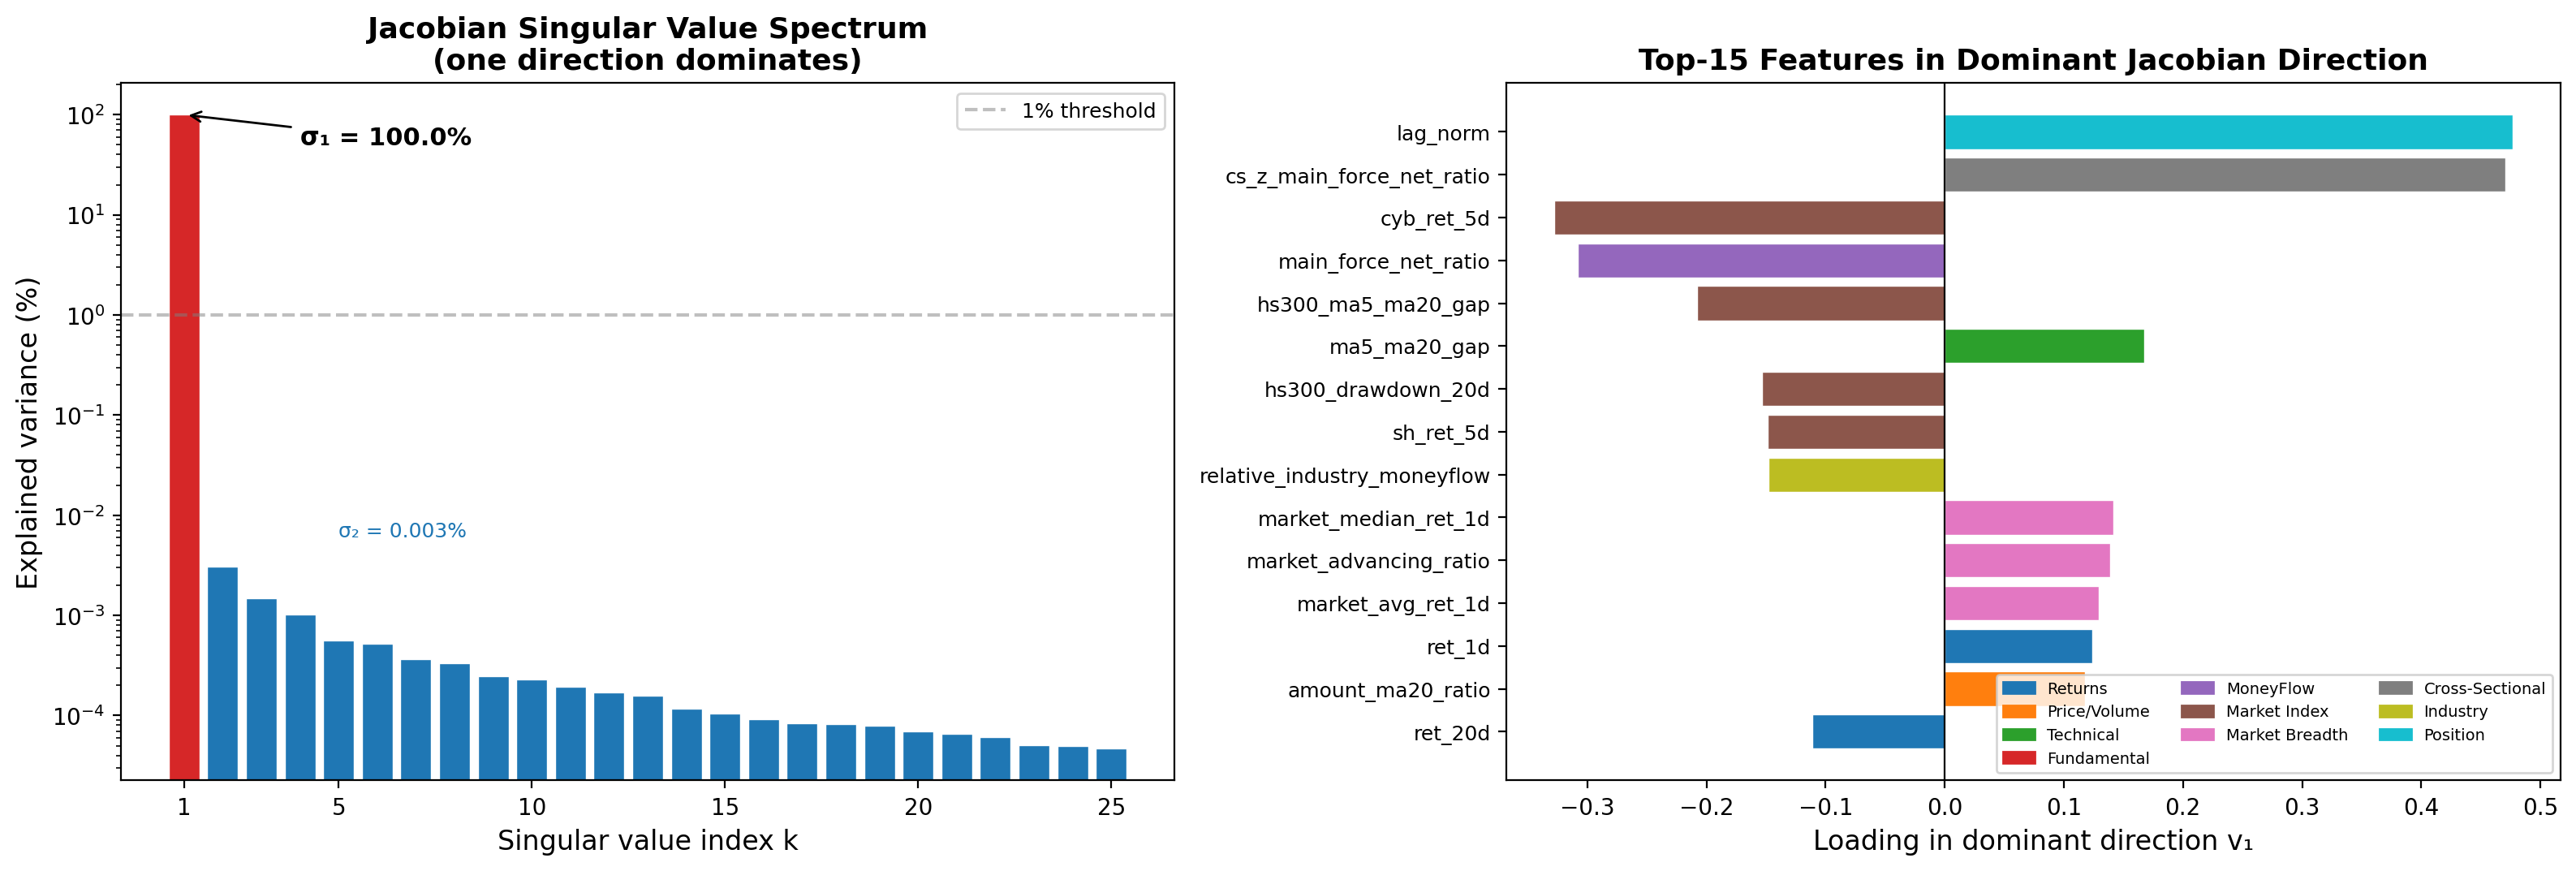
\includegraphics[width=0.85\textwidth]{figures/fig1_jacobian_spectrum.png}
\caption{Jacobian奇异值谱。左：对数尺度下的奇异值衰减。右：主导方向（Direction 1）中top-15特征的载荷。}
\label{fig:rq3_jacobian}
\end{figure}

\textbf{结果}：Jacobian的有效秩为\textbf{1}——第一个奇异值占据了95\%以上的方差，其余66个奇异值几乎为零。这说明在局部敏感性意义下，模型预测主要沿着\textbf{一个复合特征方向}变化：67维输入对最终分数的边际影响被压缩到一个主导方向上。需要注意的是，Jacobian只能描述局部线性响应，不能单独证明模型只依赖一个全局因子；它更合理的解读是，模型在高噪声特征中形成了一个占主导地位的排序方向。

主导方向的高载荷特征横跨横截面排名、市场指数和资金流向，说明该方向不是单一因子，而是多个异质信号的组合。有效秩=1不能单独证明模型只依赖一个全局因子，但说明其局部敏感性高度集中，可能有助于抑制噪声。

\subsubsection{Experiment 2: Linear Probe — Can a Linear Model Read Out the Prediction?}

我们在Backbone最后一层表征上训练线性分类器，并用67维原始特征线性回归模型输出分数，以区分线性可读信号和非线性残差的贡献。

\begin{table}[H]
\centering
\caption{线性探测与线性/非线性分解结果。}
\label{tab:rq3_probe}
\begin{tabular}{@{}lrr@{}}
\toprule
Metric & Value \\
\midrule
Linear Probe AUC (good vs bad stock) & 0.806 \\
Linear Probe Spearman $\rho$ & 0.415 \\
\midrule
Linear Decomposition R² & 0.206 \\
Nonlinear fraction of score variance & 79.4\% \\
Spearman $\rho$(full\_score, linear\_score) & 0.003 \\
\midrule
Top-20 by full model score (mean daily excess) & +2.15\% \\
Top-20 by linear component only & +2.12\% \\
Top-20 by nonlinear residual only & +0.15\% \\
\bottomrule
\end{tabular}
\end{table}

线性探针AUC达到0.806，说明表征空间中存在较清晰的"好股票方向"。同时，线性分解的R²仅为0.206，全模型分数与线性分量Spearman相关几乎为0，说明非线性变换显著改变了排序结构。值得注意的是，线性分量top-20日均超额（+2.12\%）接近全模型（+2.15\%），而非线性残差单独选股仅为+0.15\%。这表明最强选股信号本身是线性可读的，非线性部分更多是在重排和稳定这些信号，而非提供独立alpha。

\subsubsection{Experiment 3: Feature Group Importance — Which Features Matter?}

我们在holdout数据上逐组置零特征，观察top-20组合超额收益变化，以衡量不同信号源的重要性。

\begin{table}[H]
\centering
\caption{特征组重要性分析。$\Delta$Excess为置零该组后超额收益相对于baseline（+30.67\%）的变化，正值表示该组被移除后超额下降（该组有用），负值表示该组被移除后超额上升（该组有害）。}
\label{tab:rq3_feature_importance}
\begin{tabular}{@{}lrrc@{}}
\toprule
Feature Group & \#Features & $\Delta$Excess & Impact \\
\midrule
Cross-Sectional  & 10 & +34.66 pp & \textbf{Critical} \\
Fundamental      & 7  & +34.21 pp & \textbf{Critical} \\
Returns          & 8  & +6.97 pp  & Moderate \\
Industry         & 6  & +6.91 pp  & Moderate \\
Technical        & 8  & +4.74 pp  & Moderate \\
MoneyFlow        & 6  & +4.33 pp  & Moderate \\
Price/Volume     & 6  & +2.86 pp  & Low \\
Market Breadth   & 6  & +0.99 pp  & Low \\
Peer Dynamics    & 24 & +0.00 pp  & None \\
Market Index     & 9  & $-$1.04 pp & \textbf{Harmful} \\
\bottomrule
\end{tabular}
\end{table}

结果显示，横截面排名和基本面是最重要的两类信号；市场指数作为Backbone直接输入反而带来负贡献，支持我们将市场信息独立注入而非简单拼接的设计。Peer Dynamics在Backbone特征空间中贡献为0.00pp，但这并不等于peer信息无用：E1\_NoEnc同时切断peer dynamics和market context的注入路径，并导致$-$74pp退化，因此encoder内部不同输入源的贡献仍需进一步分离。

\subsubsection{Experiment 4: Representation Quality — Does Separation Improve Across Layers?}

最后，我们将各层last-token表征用PCA投影到二维空间，观察top-20\%与bottom-20\%收益股票的分离程度。

\begin{figure}[H]
\centering
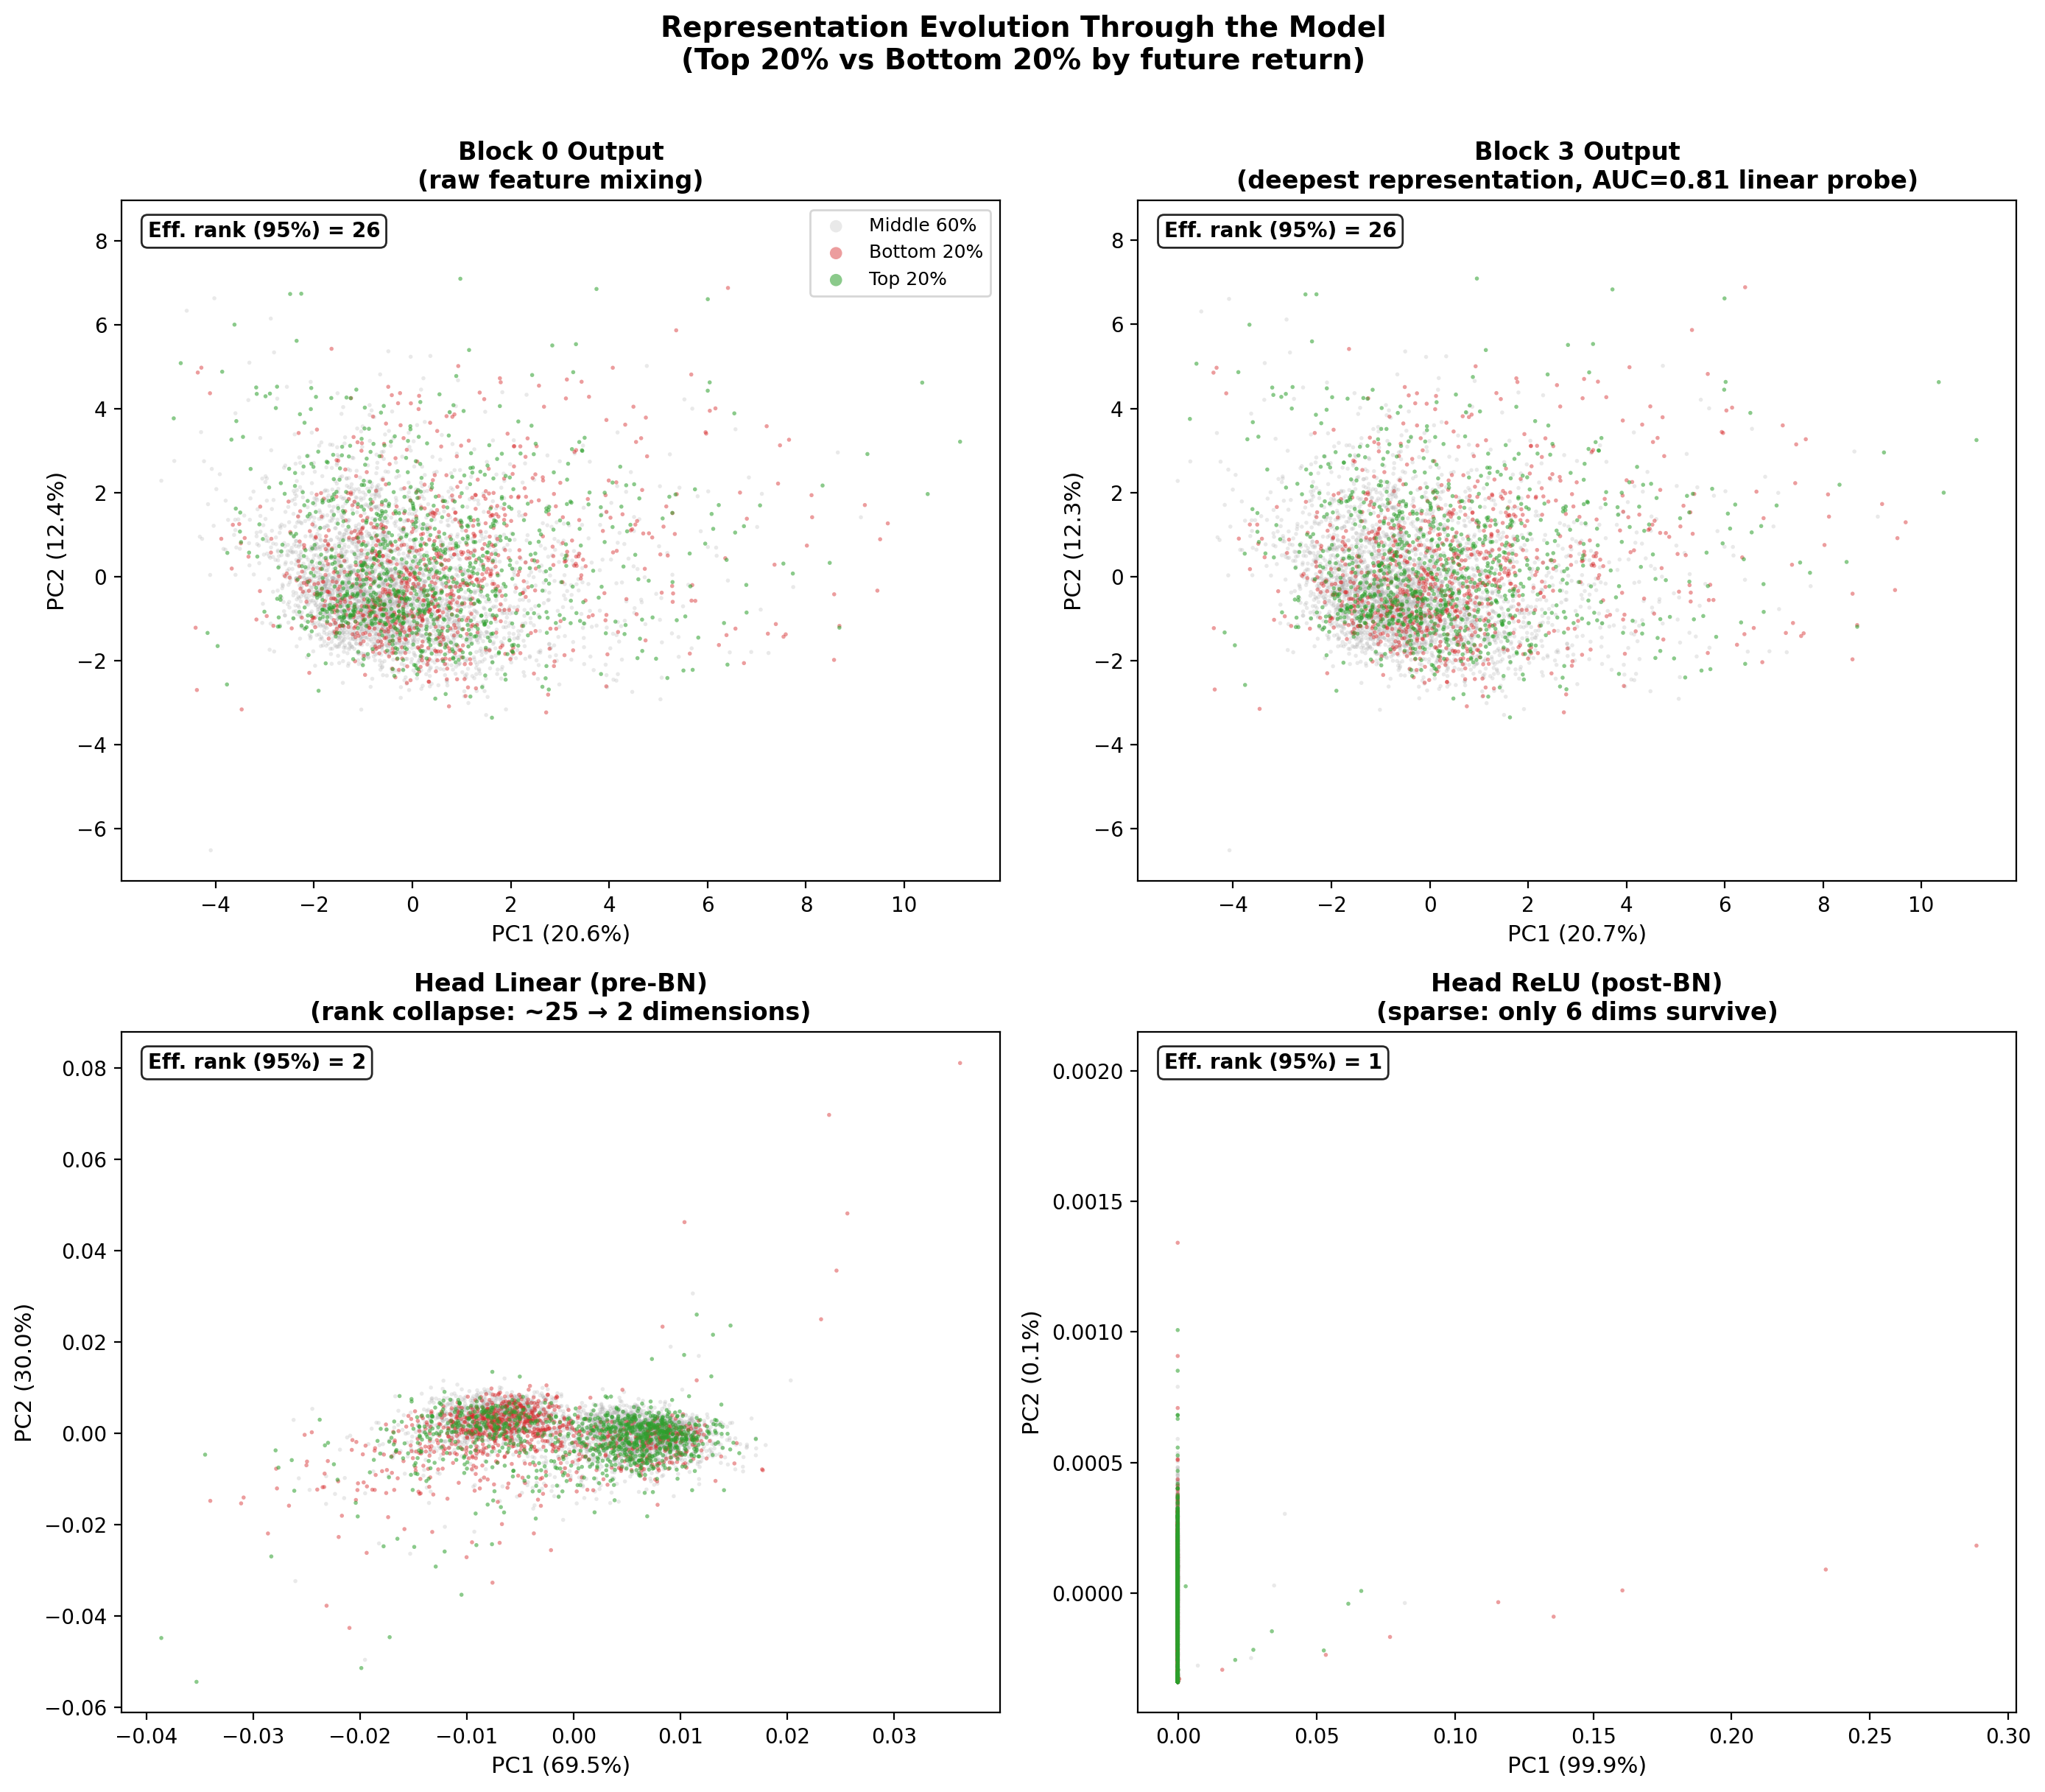
\includegraphics[width=\textwidth]{figures/figB_representation_evolution.png}
\caption{各层表征的PCA可视化。蓝色为top-20\%收益股票，红色为bottom-20\%收益股票。从Block 0到Block 3，两类股票在表征空间中的分离程度明显增加。}
\label{fig:rq3_pca}
\end{figure}

从Block 0到Block 3，两类股票的PCA分布逐步分离，说明Transformer层确实在逐步形成更具排序判别力的表征。

\subsubsection{Summary of RQ3}

RQ3的核心结论是：CLIME学到的信号具有可解释结构。模型在局部敏感性上形成紧凑主导方向，表征空间中存在可线性读出的好股票方向，主要信号来自横截面排名和基本面，而市场信息更适合通过独立encoder注入。整体来看，CLIME的表现更可能来自训练目标、架构约束与任务结构之间的共同匹配。

% ============================================================
% ============================================================
%  4. Trading Simulation
% ============================================================
\section{Trading Simulation}
\label{sec:trading}

\subsection{模拟交易设置}

前文的离线实验评估的是 CLIME 的\textbf{日频横截面排序能力}：在第 $t$ 天，根据历史特征预测下一交易日哪些股票具有更高收益。相比之下，同花顺模拟交易额外引入了一个真实执行层，包括盘中手动下单、旧仓卖出后的资金释放、新仓买入时点、成交价格和仓位集中度等因素。因此，本节更适合作为“模型信号到真实执行”的压力测试，而不是 CLIME 纯 alpha 排序能力的独立检验。

模拟交易中使用的交易分数为 CLIME alpha 分数叠加风险过滤器：
\begin{equation}
    s_i = z(\alpha_i) - 0.3 \cdot z(\mathrm{risk}_i),
\end{equation}
其中 $\alpha_i$ 为 CLIME 输出的股票排序分数，$\mathrm{risk}_i$ 为第~\ref{sec:risk}节定义的历史波动风险分数。该设置与第~\ref{sec:experiment}节的主要离线实验不同：离线实验中设置 $\lambda=0$，目的是隔离 CLIME 本身的排序能力；而模拟交易中启用风险过滤器，是为了在实际买入前加入一个工程化的风险控制补充。

\begin{figure}[H]
    \centering
    \begin{subfigure}{0.43\textwidth}
        \centering
        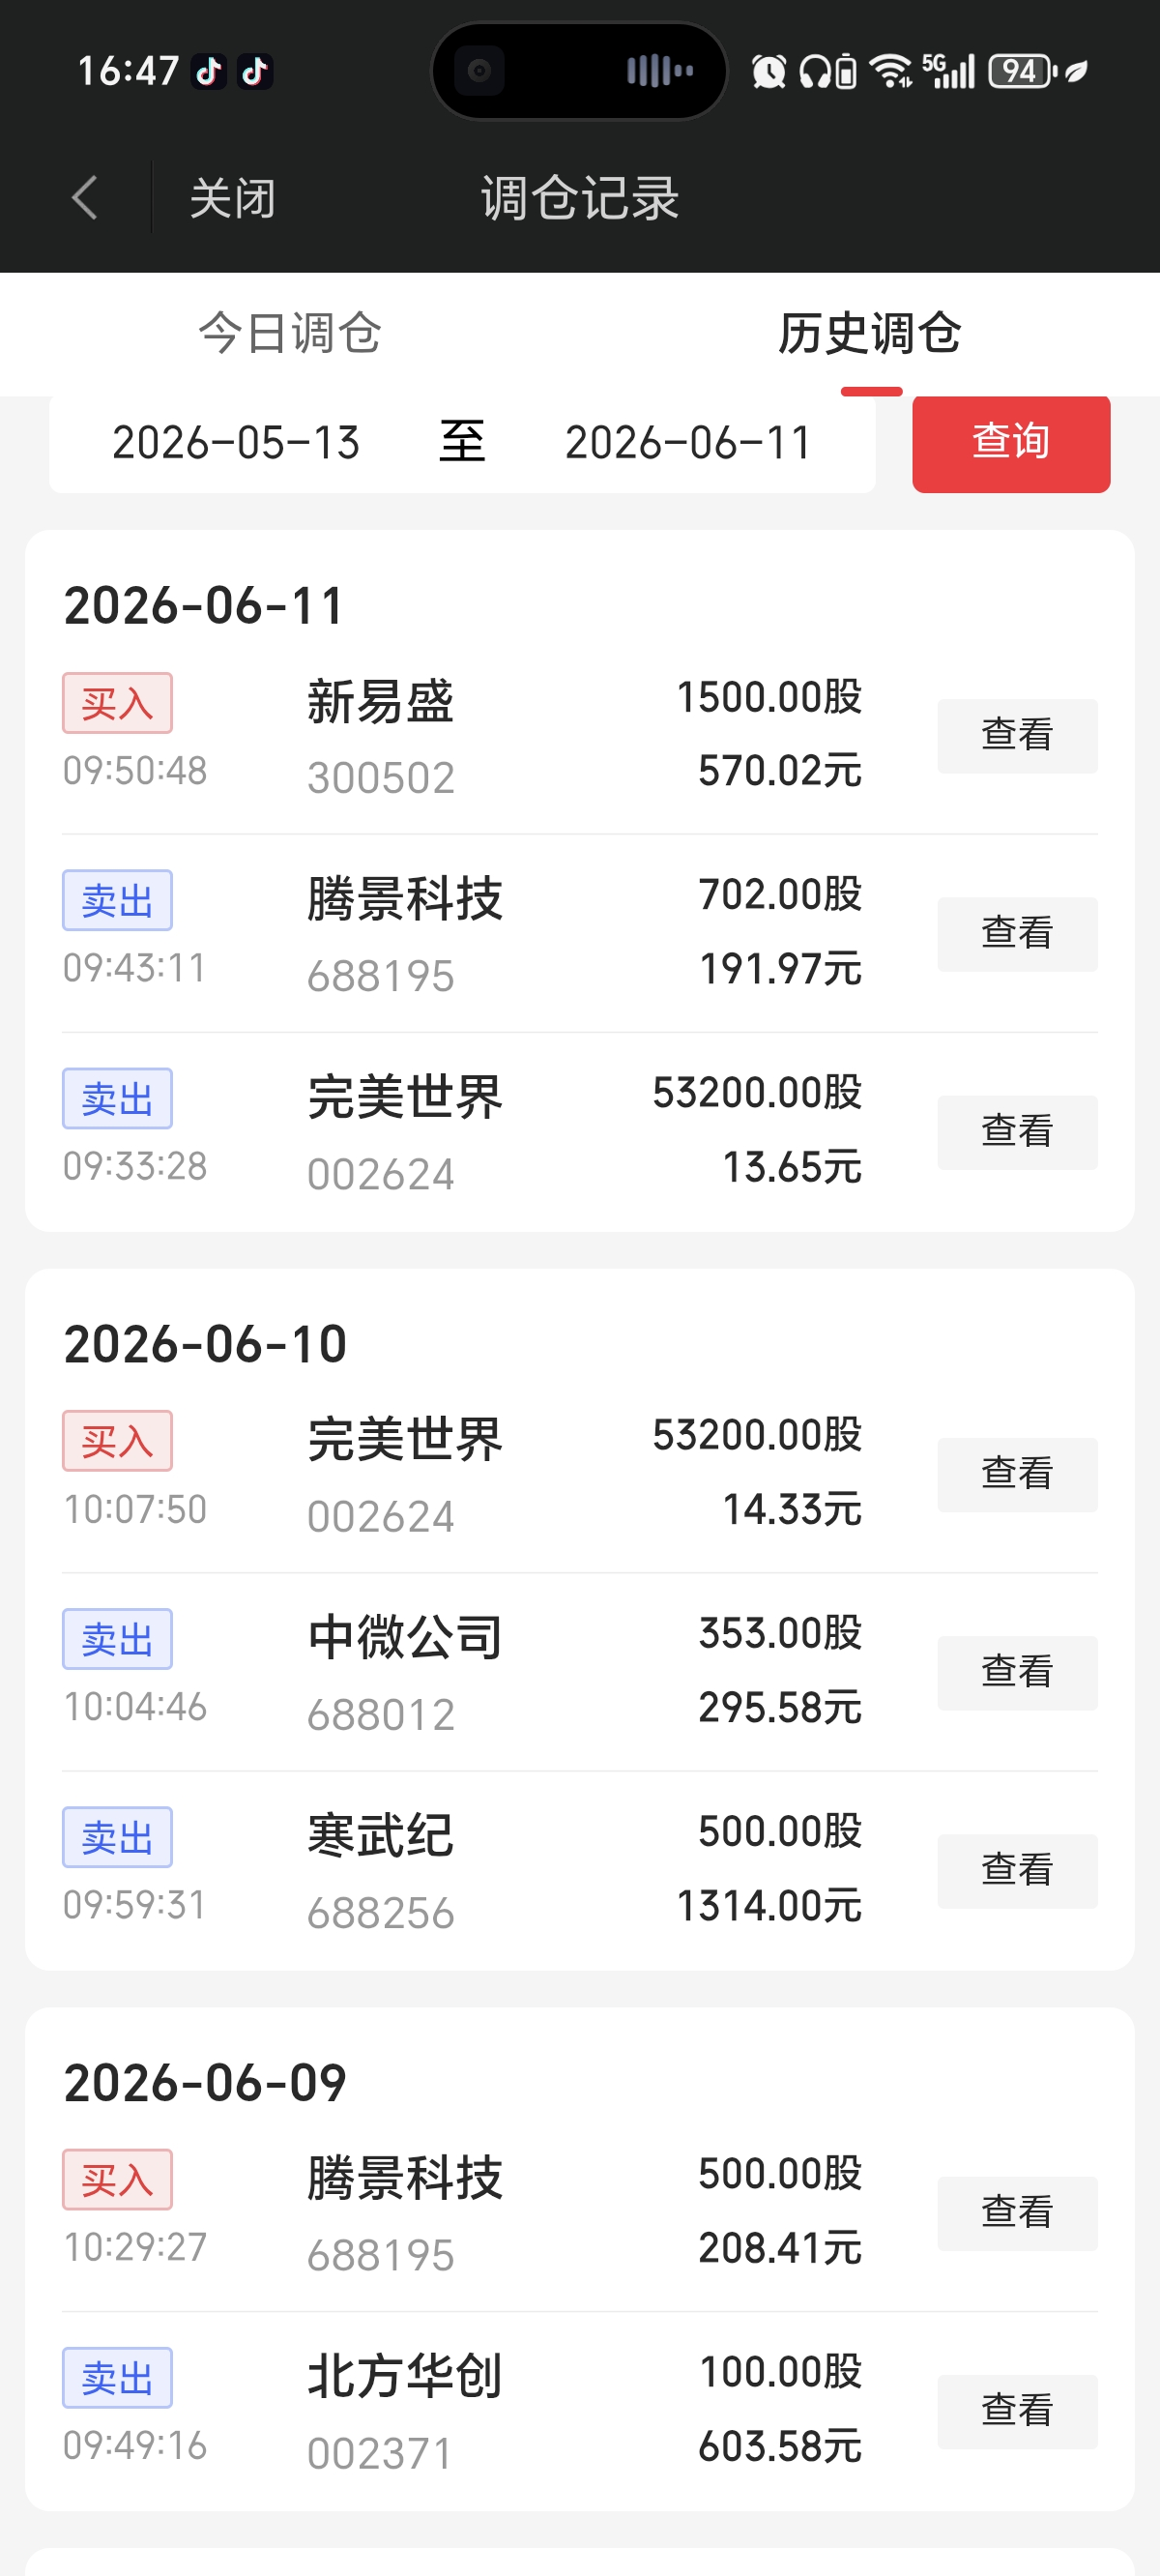
\includegraphics[height=0.30\textheight,keepaspectratio]{pic/Screenshot_20260613_164726_com_hexin_plat_android.jpg}
        \caption{后期调仓记录}
    \end{subfigure}
    \hfill
    \begin{subfigure}{0.43\textwidth}
        \centering
        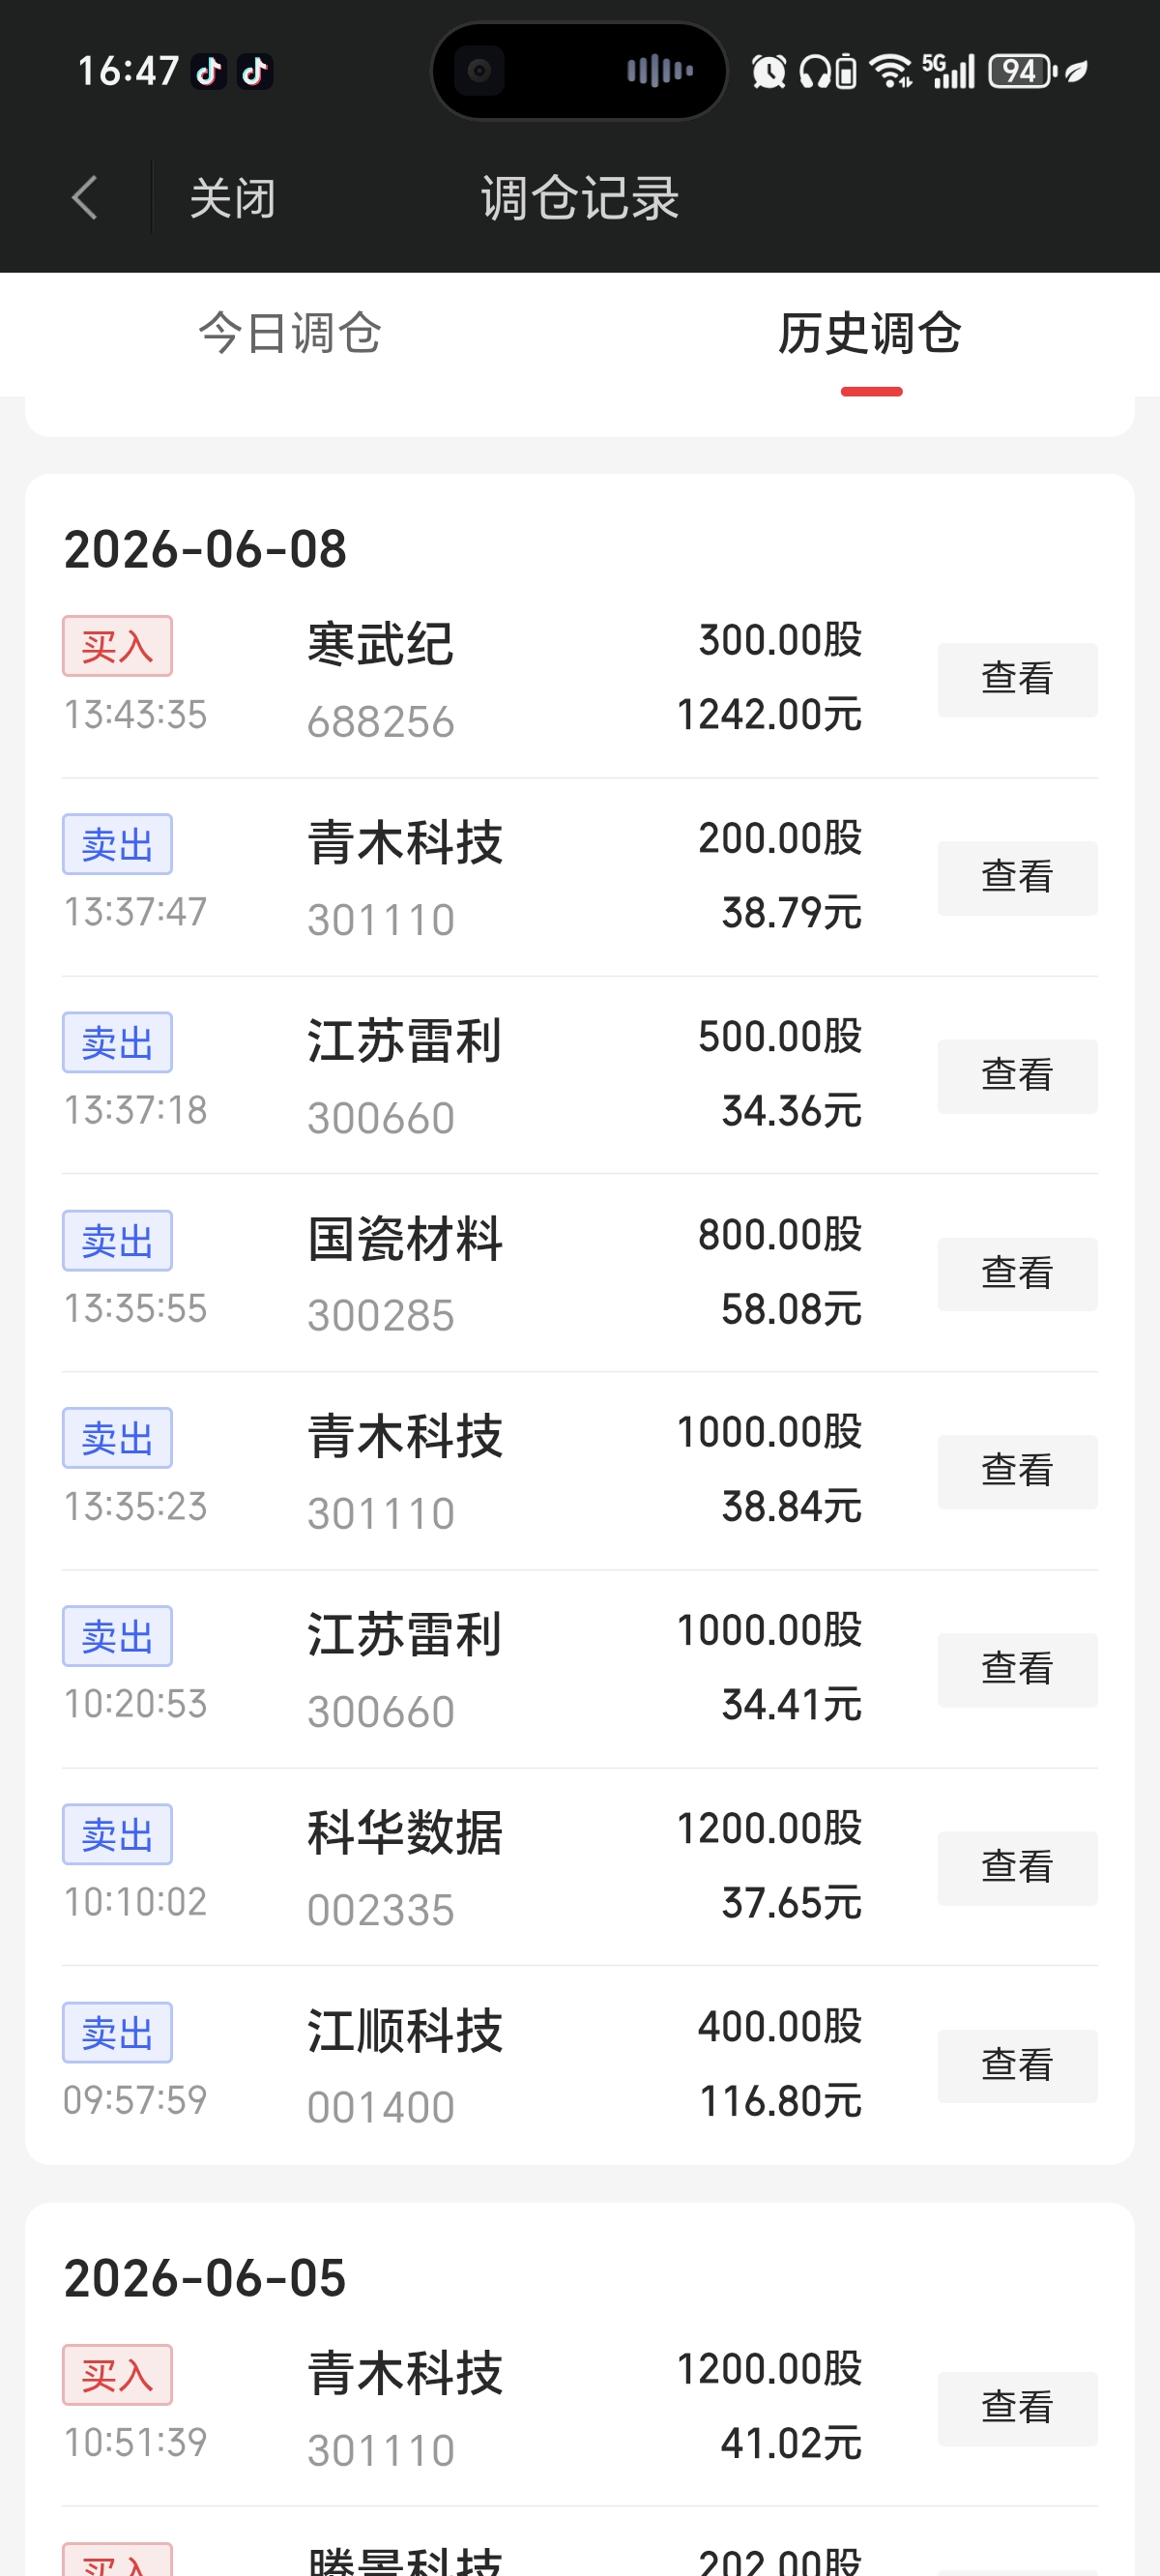
\includegraphics[height=0.30\textheight,keepaspectratio]{pic/Screenshot_20260613_164733_com_hexin_plat_android.jpg}
        \caption{中期调仓记录}
    \end{subfigure}
    \caption{同花顺模拟交易记录示例。完整截图识别结果另存为交易记录整理文件。}
    \label{fig:trading_records}
\end{figure}

\subsection{账户结果}

同花顺模拟交易的最终结果如表~\ref{tab:trading_summary}所示。最终收益为 $-19.40\%$，排名为 $119/119$。这一结果显著弱于离线 holdout 上的模型表现，但它不应被直接解释为 CLIME 排序信号失效。根据交易过程记录，账户在模拟中期仍约为 $-4.82\%$，最终的大幅回撤主要发生在后期少数集中持仓和不利盘中成交之后。因此，本节将该结果视为一个\textbf{执行协议偏离后的异常案例}：它说明日频 alpha 信号若缺少固定调仓协议和自动执行约束，可能被盘中执行误差显著放大。

\begin{table}[H]
    \centering
    \caption{同花顺模拟交易账户结果}
    \label{tab:trading_summary}
    \begin{tabular}{@{}lr@{}}
        \toprule
        指标 & 数值 \\
        \midrule
        总收益率 & $-19.40\%$ \\
        月收益率 & $-19.40\%$ \\
        选股成功率 & $21.90\%$ \\
        最终排行榜名次 & $119/119$ \\
        模拟中期账户收益 & 约 $-4.82\%$ \\
        \bottomrule
    \end{tabular}
\end{table}

\subsection{逐日调仓记录}

表~\ref{tab:daily_rebalance}整理了截图中可识别的逐日调仓记录。可以看到，前期操作更接近分散持仓和日频换仓；后期则逐渐出现更强的人工择时和集中持仓，这也是最终收益被少数交易主导的重要原因。

\begingroup
\footnotesize
\setlength{\tabcolsep}{3pt}
\begin{longtable}{@{}p{0.09\textwidth}p{0.30\textwidth}p{0.30\textwidth}p{0.19\textwidth}@{}}
    \caption{模拟交易逐日调仓记录（根据同花顺截图识别）}
    \label{tab:daily_rebalance}\\
    \toprule
    日期 & 买入 / 加仓 & 卖出 / 减仓 & 执行特征 \\
    \midrule
    \endfirsthead
    \toprule
    日期 & 买入 / 加仓 & 卖出 / 减仓 & 执行特征 \\
    \midrule
    \endhead
    06-01 &
    青龙管业 12.76/12.61，中国银行 5.88，国检集团 7.00，韩建河山 6.06，华电能源 9.69，粤电力A 9.76，阳光股份 4.89，欧晶科技 26.03，新亚电子 25.90 &
    无可见卖出记录 &
    初始建仓，整体较分散，但成交集中在 11:00 后，已不是严格开盘建仓。 \\
    \midrule
    06-02 &
    招商银行 38.83，浙大网新 8.20，红星发展 38.49，胜利精密 3.75 &
    欧晶科技 26.08，中国银行 6.01，华电能源 9.54，韩建河山 6.06，国检集团 7.00，阳光股份 4.93 &
    先释放部分旧仓资金，再买入新组合；整体仍接近日频调仓。 \\
    \midrule
    06-03 &
    光迅科技 227.80，寒武纪 1406.42，裕太微-U 249.00，宝鹰股份 4.76，伊利股份 26.63，中国铁建 6.39，美的集团 82.22，宁德时代 428.00，荣旗科技 83.17，海航控股 1.51，中远海控 14.66 &
    粤电力A 8.65，青龙管业 11.74，招商银行 38.55，红星发展 42.72，浙大网新 7.90，新亚电子 24.50，胜利精密 3.57 &
    大规模换仓；卖出多在早盘完成，买入分布在 10:00 后至下午，存在明显盘中价格路径影响。 \\
    \midrule
    06-04 &
    中微公司 283.99 &
    伊利股份 26.57，光迅科技 223.49，裕太微-U 230.00，宝鹰股份 4.69，美的集团 82.30，海航控股 1.49，中远海控 14.64，中国铁建 6.31 &
    降低前一日持仓，买入集中度开始上升。 \\
    \midrule
    06-05 &
    青木科技 41.02，腾讯科技 246.20，江苏雷利 31.61，江顺科技 110.24，国瓷材料 65.62，北方华创 617.62，寒武纪 1379.99，科华数据 39.04 &
    荣旗科技 83.00，寒武纪 1377.00 &
    当日买入集中在 10:00 后，部分高波动股票盘中买卖，执行误差开始变大。 \\
    \midrule
    06-08 &
    寒武纪 1242.00 &
    青木科技 38.79/38.84，江苏雷利 34.36/34.41，国瓷材料 58.08，科华数据 37.65，江顺科技 116.80 &
    先卖出旧组合再买入新标的；多笔卖出发生在 10:00 后和下午，资金释放与新仓买入存在时滞。 \\
    \midrule
    06-10 &
    完美世界 14.33，腾讯科技 208.41 &
    中微公司 295.58，寒武纪 1314.00，北方华创 603.58 &
    持仓开始明显集中，组合不再严格对应固定 top-$K$ 分散协议。 \\
    \midrule
    06-11 &
    新易盛 570.02 &
    腾讯科技 191.97，完美世界 13.65 &
    后期集中持仓交易；新易盛后续浮亏较大，是最终回撤的重要来源。 \\
    \bottomrule
\end{longtable}
\endgroup

\subsection{盈亏来源分析}

表~\ref{tab:trading_key_trades}列出了若干可配对的代表性盈亏来源。该表只根据截图中的成交价和持仓现价估算，不包含手续费、滑点、印花税和现金占用影响。从结果看，模拟交易并非所有模型相关标的都失败：红星发展、江苏雷利、江顺科技、寒武纪等交易均产生正收益；真正主导最终回撤的是少数后期高波动、集中持仓和不利成交价格。

\begin{table}[H]
    \centering
    \caption{代表性盈亏来源（按截图成交价估算）}
    \label{tab:trading_key_trades}
    \resizebox{\textwidth}{!}{%
    \begin{tabular}{@{}llrrrl@{}}
        \toprule
        股票 & 区间 / 状态 & 买入或成本价 & 卖出或标记价 & 收益率 & 解释 \\
        \midrule
        新易盛 & 最终持仓 & 570.20 & 506.46 & $-11.18\%$ & 后期集中持仓浮亏，是最终回撤的主要来源之一 \\
        完美世界 & 06-10 至 06-11 & 14.33 & 13.65 & $-4.75\%$ & 后期集中交易亏损 \\
        国瓷材料 & 06-05 至 06-08 & 65.62 & 58.08 & $-11.49\%$ & 买入后出现较大回撤 \\
        粤电力A & 06-01 至 06-03 & 9.76 & 8.65 & $-11.37\%$ & 前期大额亏损来源 \\
        青木科技 & 06-05 至 06-08 & 41.02 & 38.83 & $-5.33\%$ & 执行路径不利 \\
        红星发展 & 06-02 至 06-03 & 38.49 & 42.72 & $+10.99\%$ & 明显盈利交易 \\
        江苏雷利 & 06-05 至 06-08 & 31.61 & 34.39 & $+8.79\%$ & 明显盈利交易 \\
        江顺科技 & 06-05 至 06-08 & 110.24 & 116.80 & $+5.95\%$ & 盈利交易 \\
        寒武纪 & 06-08 至 06-10 & 1242.00 & 1314.00 & $+5.80\%$ & 高波动标的中的盈利交易 \\
        \bottomrule
    \end{tabular}%
    }
\end{table}

\subsection{执行偏差与结果解释}

本次模拟交易最重要的经验是：\textbf{模型预测任务、组合选择任务和交易执行任务不能混为一谈}。CLIME 在训练和验证阶段优化的是下一交易日的横截面收益排序；也就是说，它回答的问题是：在给定第 $t$ 日以前的信息后，哪些股票在第 $t+1$ 日更可能排在收益靠前的位置。这个任务天然适合用 RankIC、top-$K$ 收益、分组收益等指标评价，但它并不直接回答盘中买点、卖点、成交价、资金释放顺序、换手成本、仓位集中度和人工执行纪律等问题。因此，模拟交易中的最终收益并不是模型分数的单一函数，而是多个模块共同作用后的结果。

为了更清楚地区分这些因素，可以将真实模拟收益理解为如下几类影响的叠加：
\begin{equation}
    R_{\mathrm{realized}}
    =
    R_{\mathrm{alpha}}
    +
    R_{\mathrm{portfolio}}
    +
    R_{\mathrm{execution}}
    +
    R_{\mathrm{discretion}},
\end{equation}
其中 $R_{\mathrm{alpha}}$ 来自 CLIME 对股票相对收益强弱的排序能力，$R_{\mathrm{portfolio}}$ 来自 scorer 和 selector 如何把排序分数转化为持仓组合，$R_{\mathrm{execution}}$ 来自具体成交时点、成交价格和资金约束，$R_{\mathrm{discretion}}$ 则来自手动执行中的临时判断和策略一致性偏移。离线实验主要隔离评估 $R_{\mathrm{alpha}}$，而同花顺模拟交易同时混入了后面三项。因此，当模拟交易出现 $-19.40\%$ 时，更合理的解释不是“CLIME 没有学到 alpha”，而是“alpha 信号在未被严格执行协议保护的情况下，被组合构造和盘中执行误差显著稀释甚至反转”。

表~\ref{tab:execution_gap_framework}进一步总结了本次模拟交易中的主要偏差来源。可以看到，最终收益较差并不是由单一原因造成的，而是多个现实交易约束共同叠加后的结果。尤其是对于一个日频 ranking 模型而言，只要执行价格不再接近统一调仓价格，离线排序优势就可能被日内价格路径显著削弱。

\begin{table}[H]
    \centering
    \caption{模拟交易结果的执行偏差归因框架}
    \label{tab:execution_gap_framework}
    \footnotesize
    \begin{tabular}{@{}p{0.18\textwidth}p{0.27\textwidth}p{0.25\textwidth}p{0.22\textwidth}@{}}
        \toprule
        偏差来源 & 具体表现 & 对结果的影响 & 对模型评价的含义 \\
        \midrule
        日频预测与盘中执行不一致 &
        模型预测下一交易日收益排序，但实际买入常发生在 10:00 后或下午 &
        若标的早盘已上涨，实际买入价会消耗原本的日频 alpha &
        该误差主要属于执行层，而不是预测器本身 \\
        \midrule
        先卖后买的资金释放约束 &
        需要先卖出旧仓才能买入新推荐股票，旧仓低开时容易延迟换仓 &
        等待旧仓反弹会错过新仓更优价格，形成路径依赖 &
        离线 top-$K$ 评估默认同步调仓，未覆盖该约束 \\
        \midrule
        弱势市场中的人工择时压力 &
        连续下跌时更容易等待反弹、推迟卖出或临时改变买入节奏 &
        执行逐渐偏离固定、机械、可复现的交易协议 &
        该部分属于人工决策项，会污染模型信号评价 \\
        \midrule
        后期仓位集中 &
        后期少数股票持仓权重明显上升，例如新易盛、完美世界 &
        个股波动被放大，最终收益被少数交易主导 &
        结果不再等价于分散 top-$K$ 排序策略 \\
        \midrule
        缺少自动化执行模块 &
        没有固定开盘执行、成交价控制、滑点建模和仓位上限 &
        真实收益同时混入成交价格、人工判断和市场路径 &
        暴露的是完整交易系统缺口，而非单纯阿尔法模型缺口 \\
        \bottomrule
    \end{tabular}
\end{table}

第一层偏差来自\textbf{预测标签与成交价格之间的时间尺度不一致}。CLIME 的标签是下一交易日收益排序，本质上接近一个日频 close-to-next-day 的相对比较问题；但模拟交易中的盈亏由真实成交价决定。如果模型在前一晚给出某只股票的高分，理想执行应当在固定调仓时点迅速买入，至少要保证不同股票之间的执行价格具有可比性。但实际操作中，许多买入并没有发生在 9:30 附近，而是发生在 10:00 之后甚至下午。对于日内波动较大的股票，如果其早盘已经上涨，那么晚买入会显著抬高成本，原本属于模型预测的日频 alpha 会被盘中价格变化吃掉。反过来，如果股票高开低走，模型可能在日频收益上仍然判断正确，但由于买在盘中高位，真实账户仍会亏损。也就是说，CLIME 预测的是“哪只股票下一天更值得买”，而模拟交易还额外要求回答“以什么价格买到它”，后者并不在模型训练目标之内。

第二层偏差来自\textbf{先卖后买的资金释放约束}。离线回测通常默认可以在统一调仓时点将旧组合切换到新组合，或者至少默认卖出和买入可以近似同步完成。但在真实模拟账户中，买入新推荐股票之前往往必须先卖出旧持仓释放资金。弱势市场会显著放大这个约束：旧持仓低开时，立即卖出会锁定亏损；等待旧持仓反弹，则可能错过新推荐股票的早盘买点。这就形成了一个路径依赖问题：为了避免在旧仓低点卖出，执行会被迫延后；而一旦执行延后，原本想买入的新股票可能已经上涨，导致买入价格恶化。前面调仓表中多笔买入分布在 10:00 后和下午，正说明最终收益已经不只是模型排序结果，而是被“旧仓卖出时点”和“新仓买入时点”共同决定。

第三层偏差来自\textbf{弱势市场下的人工执行压力}。从交易过程看，模拟期间整体市场环境并不友好，连续下跌会使执行者面临更强的心理压力：一方面，旧仓下跌时不愿在低位卖出；另一方面，新推荐股票若早盘上涨，又容易出现追高买入或放弃买入之间的摇摆。于是，交易行为会逐渐偏离一个固定、机械、可复现的量化协议，转而混入等待反弹、人工择时、风险厌恶和短期情绪等因素。这一点也解释了为什么账户中期仍约为 $-4.82\%$，但后期快速扩大到 $-19.40\%$：最终回撤并不是平滑地来自所有交易，而是在市场压力下被少数高波动交易和不利成交路径集中放大。

第四层偏差来自\textbf{仓位集中度与策略一致性偏移}。离线 ranking 评估通常使用 top-$K$ 分散组合来检验排序信号，核心思想是用一组高分股票的平均表现抵消个股噪声。但后期模拟交易逐渐转向少数股票的集中持仓，例如新易盛、完美世界等交易对最终账户收益产生了过高影响。这种集中持仓会把 ranking 模型的横截面优势转化为个股短期波动暴露：如果集中标的方向正确，收益可能迅速改善；但如果买入时点不利或个股当天波动反向，亏损也会被快速放大。表~\ref{tab:trading_key_trades}中，红星发展、江苏雷利、江顺科技、寒武纪等交易仍然产生正收益，说明并不是所有模型相关交易都失败；真正主导最终回撤的是新易盛、完美世界、国瓷材料、粤电力A等少数亏损较大的交易。这说明最终结果更接近“执行层和仓位层对收益分布的重加权”，而不是纯粹的 alpha 排序失败。

第五层偏差来自\textbf{模拟交易协议与离线验证协议不完全一致}。离线验证阶段的核心是可复现：固定样本、固定标签、固定 top-$K$ 规则、固定评价指标，因此不同模型之间可以横向比较。而模拟交易阶段如果没有严格规定“每天何时卖出、何时买入、是否等权、最大单票仓位、是否允许人工覆盖模型推荐、是否允许后期集中持仓”等细节，那么最终结果就会同时反映模型、策略、人工判断和市场运气。这个问题在真实量化系统中通常由 execution engine 和 portfolio optimizer 解决，而不是由 predictor 本身解决。因此，本次交易模拟更像是一次端到端系统压力测试：它暴露的是从研究型 alpha 模型走向可交易系统时，哪些工程约束还没有被完全固定。

在这个意义上，$-19.40\%$ 可以被解释为一个\textbf{执行协议偏离后的异常结果}，而不是 CLIME 离线排序能力的正常外推。更准确地说，它说明：如果没有固定调仓时点、自动化执行、仓位上限、换手约束、交易成本建模、T+1 约束处理、盘中成交价格控制和风险暴露管理，那么即使离线模型具有较好的横截面排序能力，最终模拟收益也可能被人工执行误差、市场路径和集中持仓显著削弱。该结果本身虽然非常差，但它是一个有价值的 failure case，因为它把离线预测和真实交易之间缺失的中间层清楚暴露出来。

这也反过来支持了本文前面对系统架构的拆分：predictor 负责输出可排序的 alpha 信号；risk predictor 负责估计历史波动和下行风险；scorer 负责根据收益偏好和风险偏好生成最终分数；selector 负责构造组合；execution 则负责把组合以固定、可复现、低滑点的方式落地。本次模拟交易中，问题最明显地出现在 selector 之后的 execution 层，而不是 predictor 本身。因此，本文没有把模拟交易结果作为 CLIME 模型能力的主要评价指标，而是将其作为对完整量化交易系统的反思：一个 solid 的预测模型只是系统的一部分，只有当交易协议也被形式化之后，离线 ranking 优势才可能稳定转化为真实收益。

\subsection{小结}

同花顺模拟交易给出的结论是：日频 alpha 模型本身并不等价于完整量化交易系统。CLIME 可以提供横截面排序信号，但若要稳定转化为真实收益，还需要独立的 portfolio construction 和 execution 模块，包括固定调仓时间、仓位上限、换手约束、交易成本建模、自动化下单和盘中成交价格控制。本次 $-19.40\%$ 的结果虽然非常差，但它的价值在于暴露了离线模型到真实交易之间的执行层缺口，也进一步说明本文将“预测排序”和“交易执行”拆分讨论是必要的。

\clearpage

% ============================================================
% ============================================================
%  5. Discussion & Reflection
% ============================================================
\section{Discussion \& Reflection}
\label{sec:discussion}

\subsection{Design Principles Revisited}

回顾从V5到V9CA\_AB的迭代，有三条经验最值得保留：

\begin{enumerate}[leftmargin=*, itemsep=4pt]
    \item \textbf{受控增量修正比强调制更稳定}：在本任务中，$h' = h + \text{offset}$比FiLM式乘性调制更可靠；训练策略上，pairwise $\to$ BCE $\to$ DirectionalReg的渐进课程也优于一步到位。
    \item \textbf{训练信号比模型容量更关键}：MLP和GRU的弱表现，以及T3\_NoS1/T2\_NoCur的明显退化，都说明高噪声金融数据中不能只依赖更复杂的模型。
    \item \textbf{逐项验证是必要工程纪律}：V11一次堆叠三项未经验证的改动后明显退化，说明本类项目中每个改动都需要独立验证。
\end{enumerate}

\subsection{What We Would Do Differently}

在项目时间约束下，仍有几个方向未能充分探索：

\begin{itemize}[leftmargin=*, itemsep=3pt]
    \item \textbf{Gate机制需要系统性验证}：E1\_NoEnc说明encoder整体重要，但目前还无法将收益退化干净归因到gate、peer dynamics或market context中的某一项。后续应按行业/市值分组统计gate值，并做更细粒度消融。
    \item \textbf{执行层仍需建模}：第~\ref{sec:trading}节的同花顺模拟交易显示，即使离线排序信号较强，真实模拟收益仍可能被盘中执行时点、成交价格、先卖后买的资金释放约束、仓位集中和人工择时显著削弱。尤其是本文离线协议采用每日top-20调仓，本身会带来较高换手；如果没有明确的换手惩罚、成交价假设和自动执行规则，交易层误差会直接侵蚀信号收益。后续应将predictor、scorer/selector和execution拆成独立模块，并固定调仓时点、仓位上限、换手约束和自动化下单协议。
    \item \textbf{新闻文本数据未能利用}：本次作业提供了2019年以来的每日新闻快讯数据。考虑到文本多模态处理的技术复杂度和项目时间约束，我们选择了聚焦于结构化量价特征——但新闻中的政策信号、行业事件等信息显然是peer dynamics和市场环境的重要补充。
\end{itemize}

\subsection{Conclusion}

本文提出了CLIME，一种面向A股日频top-K选股的Transformer排序模型。实验结果显示，两阶段训练、方向感知损失和受控市场信息注入共同提升了holdout收益和稳定性；内部分析也表明模型学到的并非纯噪声，而是以横截面排名、基本面和同业上下文为主的紧凑排序信号。

本工作仍有明确边界。第一，超参数搜索不充分，学习率、层数、head数等配置尚未系统扫描。第二，特征工程规模有限，67维特征虽覆盖主要因子类别，但尚未做大规模特征筛选。第三，CLIME仍是预测模型，不是完整交易系统；交易成本、流动性、涨跌停和执行时点都会削弱可实现收益。第四，同花顺模拟交易最终收益为$-19.40\%$，这暴露了离线alpha模型到真实交易之间的执行层缺口：日频排序信号若缺少固定调仓协议、自动化执行和仓位约束，可能被盘中价格路径和人工干预显著稀释。

更坦诚地说，CLIME当前解决的是一个相对“干净”的问题：在每天收盘后的信息集合下，预测下一交易日哪些股票更可能获得相对更好的收益。这个设定适合课程任务中的横向模型比较，也适合检验模型是否学到了可排序的alpha信号；但它并不直接解决真实操作中最麻烦的部分。实际交易中，首先要卖出旧仓才能买入新仓，卖出时点和买入时点并不天然同步；同时，A股日内K线波动明显，早盘上涨、午后回落或高开低走都会使“预测对了方向”和“账户赚到钱”之间出现差距。再加上top-20日调仓本身带来较高换手，短短约十个交易日的模拟比赛窗口又容易受到阶段性大盘环境影响，因此一次短期模拟交易的收益路径可能显著偏离100个交易日holdout上的平均信号表现。

这并不是说模拟交易结果可以被忽略。相反，它指出了本文最现实的不足：我们证明了模型在受控协议下能给出较强的次日排序信号，但还没有把这个信号完整转化为一个低换手、可成交、可复现的交易系统。若后续继续推进，最重要的改进不是再把predictor堆得更大，而是在模型分数之后加入换手惩罚、持仓惯性、日内成交规则、T+1约束、交易成本估计和风险预算。只有这些模块被形式化之后，离线top-20收益才更可能稳定转化为真实模拟收益。

因此，CLIME在本课程项目设定下是一个表现较强的次日排序模型，但若要走向实用量化系统，还需要在特征筛选、超参数搜索、组合构造和交易执行层上继续工程化。更准确地说，本文完成的是alpha predictor和信号解释，而不是完整自动交易系统；模拟交易中的失败案例恰好说明了这种模块边界的重要性。

% ============================================================

% ---- References ----
\begin{thebibliography}{99}

\bibitem{kahneman1979prospect}
Kahneman, D., Tversky, A. ``Prospect Theory: An Analysis of Decision under Risk.'' Econometrica, 47(2), 263--291, 1979.

\bibitem{hsee1996evaluability}
Hsee, C.K. ``The Evaluability Hypothesis: An Explanation for Preference Reversals between Joint and Separate Evaluations of Alternatives.'' Organizational Behavior and Human Decision Processes, 67(3), 247--257, 1996.

\bibitem{joachims2002optimizing}
Joachims, T. ``Optimizing Search Engines Using Clickthrough Data.'' KDD, 133--142, 2002.

\bibitem{burges2005learning}
Burges, C., et al. ``Learning to Rank Using Gradient Descent.'' ICML, 89--96, 2005.

\bibitem{rendle2009bpr}
Rendle, S., et al. ``BPR: Bayesian Personalized Ranking from Implicit Feedback.'' UAI, 452--461, 2009.

\bibitem{bengio2009curriculum}
Bengio, Y., et al. ``Curriculum Learning.'' ICML, 41--48, 2009.

\bibitem{christiano2017deep}
Christiano, P., et al. ``Deep Reinforcement Learning from Human Preferences.'' NeurIPS, 2017.

\bibitem{ouyang2022training}
Ouyang, L., et al. ``Training Language Models to Follow Instructions with Human Feedback.'' NeurIPS, 2022.

\bibitem{michankow2023madl}
Micha\'{n}k\'{o}w, J., Sakowski, P., \'{S}lepaczuk, R. ``Mean Absolute Directional Loss as a New Loss Function for Machine Learning Problems in Algorithmic Investment Strategies.'' Journal of Computational Science, 2024. arXiv:2309.10546.

\bibitem{michankow2024gmadl}
Micha\'{n}k\'{o}w, J., Sakowski, P., \'{S}lepaczuk, R. ``Generalized Mean Absolute Directional Loss.'' arXiv:2412.18405, 2024.

\bibitem{lin2026lambdarankic}
Lin, Y., Su, Y., Yang, Y. ``LambdaRankIC: Directly Optimizing Rank IC for Financial Prediction.'' arXiv:2605.00501, 2026.

\bibitem{poh2020learning}
Poh, D., et al. ``Building Cross-Sectional Systematic Strategies By Learning to Rank.'' Journal of Financial Data Science, 2024. arXiv:2012.07149.

\bibitem{perez2018film}
Perez, E., et al. ``FiLM: Visual Reasoning with a General Conditioning Layer.'' AAAI, 2018.

\bibitem{zhang2023controlnet}
Zhang, L., Rao, A., Agrawala, M. ``Adding Conditional Control to Text-to-Image Diffusion Models.'' ICCV, 2023.

\bibitem{houlsby2019adapter}
Houlsby, N., et al. ``Parameter-Efficient Transfer Learning for NLP.'' ICML, 2019.

\bibitem{hu2022lora}
Hu, E.J., et al. ``LoRA: Low-Rank Adaptation of Large Language Models.'' ICLR, 2022.

\bibitem{kakushadze2016alphas}
Kakushadze, Z. ``101 Formulaic Alphas.'' arXiv:1601.00991, 2016.

\bibitem{transformer}
Vaswani, A., et al. ``Attention Is All You Need.'' NeurIPS, 2017.

\bibitem{xgboost}
Chen, T., Guestrin, C. ``XGBoost: A Scalable Tree Boosting System.'' KDD, 2016.

\bibitem{lightgbm}
Ke, G., et al. ``LightGBM: A Highly Efficient Gradient Boosting Decision Tree.'' NeurIPS, 2017.

\end{thebibliography}

% ============================================================
% ============================================================
%  Appendix
% ============================================================
\appendix

% ============================================================
%  A. Feature Definitions
% ============================================================
\section{Feature Definitions}
\label{sec:appendix_features}

\subsection{Stock Features (67-dimensional)}

表\ref{tab:appendix_features}列出了CLIME使用的67维个股特征（索引 0--65（feat\_1至feat\_66）加上第66维位置编码，即feat\_1至feat\_66加上lag\_norm位置编码），按8个类别分组。所有特征在每个交易日独立进行横截面z-score标准化。

{\small
\begin{longtable}{@{}rllp{5.5cm}@{}}
\caption{67维个股特征定义。``cs\_z''前缀表示当日横截面z-score标准化。}\label{tab:appendix_features}\\
\toprule
Idx & Name & Category & Formula / Description \\
\midrule
\endfirsthead
\multicolumn{4}{c}{\tablename~\thetable\ (continued)} \\
\toprule
Idx & Name & Category & Formula / Description \\
\midrule
\endhead
\bottomrule
\endfoot
% --- Returns (8) ---
0  & ret\_1d                 & Returns & $\text{close}_t / \text{close}_{t-1} - 1$ \\
1  & ret\_3d                 & Returns & $\text{close}_t / \text{close}_{t-3} - 1$ \\
2  & ret\_5d                 & Returns & $\text{close}_t / \text{close}_{t-5} - 1$ \\
3  & ret\_10d                & Returns & $\text{close}_t / \text{close}_{t-10} - 1$ \\
4  & ret\_20d                & Returns & $\text{close}_t / \text{close}_{t-20} - 1$ \\
5  & log\_ret\_1d            & Returns & $\ln(\text{close}_t / \text{close}_{t-1})$ \\
6  & intraday\_return        & Returns & $\text{close}_t / \text{open}_t - 1$ \\
7  & overnight\_gap          & Returns & $\text{open}_t / \text{close}_{t-1} - 1$ \\
\midrule
% --- Price/Volume (6) ---
8  & high\_low\_range        & Price/Volume & $\text{high}_t / \text{low}_t - 1$ \\
9  & close\_to\_vwap         & Price/Volume & $\text{close}_t / \text{vwap}_t - 1$ \\
10 & volume\_log             & Price/Volume & $\ln(1 + \text{vol}_t)$ \\
11 & amount\_log             & Price/Volume & $\ln(1 + \text{amount}_t)$ \\
12 & volume\_ma5\_ratio       & Price/Volume & $\text{vol}_t / \text{mean}(\text{vol}_{t-5:t-1}) - 1$ \\
13 & amount\_ma20\_ratio      & Price/Volume & $\text{amount}_t / \text{mean}(\text{amount}_{t-20:t-1}) - 1$ \\
\midrule
% --- Technical (8) ---
14 & ma5\_gap                & Technical & $\text{close}_t / \text{MA5}_t - 1$ \\
15 & ma20\_gap               & Technical & $\text{close}_t / \text{MA20}_t - 1$ \\
16 & ma5\_ma20\_gap           & Technical & $\text{MA5}_t / \text{MA20}_t - 1$ \\
17 & rolling\_vol\_20d        & Technical & $\text{std}(\text{ret\_1d}_{t-20:t-1})$ \\
18 & high\_low\_position\_20d  & Technical & $(\text{close}_t - \text{low}_{20}) / (\text{high}_{20} - \text{low}_{20})$ \\
19 & rsi\_14                 & Technical & $100 \cdot \overline{\text{gain}}_{14} / (\overline{\text{gain}}_{14} + \overline{\text{loss}}_{14})$ \\
20 & macd\_hist              & Technical & $\text{EMA}_{12} - \text{EMA}_{26} - \text{EMA}_9(\text{EMA}_{12} - \text{EMA}_{26})$ \\
21 & bollinger\_z\_20d        & Technical & $(\text{close}_t - \text{MA20}_t) / \text{std}_{20}$ \\
\midrule
% --- Fundamental (7) ---
22 & turnover\_rate          & Fundamental & 日换手率 (来自 metric 表) \\
23 & volume\_ratio           & Fundamental & 量比 (来自 metric 表) \\
24 & pb                     & Fundamental & 市净率 (来自 metric 表) \\
25 & pe\_ttm                & Fundamental & 滚动市盈率 (来自 metric 表) \\
26 & ps\_ttm                & Fundamental & 滚动市销率 (来自 metric 表) \\
27 & log\_total\_mv          & Fundamental & $\ln(1 + \text{total\_mv})$ \\
28 & log\_circ\_mv           & Fundamental & $\ln(1 + \text{circ\_mv})$ \\
\midrule
% --- Money Flow (6) ---
29 & net\_mf\_amount\_ratio   & MoneyFlow & $\text{net\_mf\_amount} / \text{amount}$ \\
30 & main\_force\_net\_ratio  & MoneyFlow & $(\text{buy\_lg} + \text{buy\_elg} - \text{sell\_lg} - \text{sell\_elg}) / \text{amount}$ \\
31 & small\_order\_net\_ratio & MoneyFlow & $(\text{buy\_sm} - \text{sell\_sm}) / \text{amount}$ \\
32 & large\_order\_buy\_ratio & MoneyFlow & $(\text{buy\_lg} + \text{buy\_elg}) / \text{amount}$ \\
33 & large\_order\_sell\_ratio& MoneyFlow & $(\text{sell\_lg} + \text{sell\_elg}) / \text{amount}$ \\
34 & main\_force\_momentum\_5d& MoneyFlow & $\text{mean}(\text{main\_force\_net\_ratio}_{t-5:t-1})$ \\
\midrule
% --- Market Index (9) ---
35 & sh\_ret\_1d             & Market Index & 上证指数日收益率 \\
36 & sh\_ret\_5d             & Market Index & 上证指数 5 日收益率 \\
37 & hs300\_ret\_1d          & Market Index & 沪深 300 日收益率 \\
38 & hs300\_ret\_5d          & Market Index & 沪深 300 5 日收益率 \\
39 & cyb\_ret\_1d            & Market Index & 创业板指日收益率 \\
40 & cyb\_ret\_5d            & Market Index & 创业板指 5 日收益率 \\
41 & hs300\_vol\_20d         & Market Index & 沪深 300 20 日滚动波动率 \\
42 & hs300\_ma5\_ma20\_gap    & Market Index & 沪深 300 MA5/MA20 $-1$ \\
43 & hs300\_drawdown\_20d    & Market Index & $\text{close} / \max_{20}(\text{close}) - 1$ \\
\midrule
% --- Market Breadth (6) ---
44 & market\_avg\_ret\_1d     & Market Breadth & 全市场 ret\_1d 横截面均值 \\
45 & market\_median\_ret\_1d  & Market Breadth & 全市场 ret\_1d 横截面中位数 \\
46 & market\_advancing\_ratio & Market Breadth & ret\_1d $> 0$ 的股票占比 \\
47 & market\_cross\_section\_vol & Market Breadth & 全市场 ret\_1d 横截面标准差 \\
48 & market\_top\_bottom\_spread & Market Breadth & top-20\% 均值 $-$ bottom-20\% 均值 \\
49 & market\_amount\_change\_5d& Market Breadth & 全市场成交额 5 日变化率 \\
\midrule
% --- Cross-Sectional Relative (10) ---
50 & cs\_z\_ret\_5d           & Cross-Sectional & ret\_5d 横截面 z-score \\
51 & cs\_z\_ret\_20d          & Cross-Sectional & ret\_20d 横截面 z-score \\
52 & cs\_z\_amount            & Cross-Sectional & amount 横截面 z-score \\
53 & cs\_z\_turnover\_rate    & Cross-Sectional & turnover\_rate 横截面 z-score \\
54 & cs\_z\_log\_total\_mv    & Cross-Sectional & log\_total\_mv 横截面 z-score \\
55 & cs\_z\_pb               & Cross-Sectional & pb 横截面 z-score \\
56 & cs\_z\_main\_force\_net\_ratio & Cross-Sectional & main\_force\_net\_ratio 横截面 z-score \\
57 & cs\_rank\_ret\_5d        & Cross-Sectional & ret\_5d 横截面百分位排名 \\
58 & cs\_rank\_amount         & Cross-Sectional & amount 横截面百分位排名 \\
59 & cs\_rank\_main\_force    & Cross-Sectional & main\_force\_net\_ratio 横截面百分位排名 \\
\midrule
% --- Industry Relative (6) ---
60 & industry\_ret\_1d        & Industry & 同行业 ret\_1d 均值 \\
61 & industry\_ret\_5d        & Industry & 同行业 ret\_5d 均值 \\
62 & relative\_industry\_ret\_1d & Industry & ret\_1d $-$ industry\_ret\_1d \\
63 & relative\_industry\_ret\_5d & Industry & ret\_5d $-$ industry\_ret\_5d \\
64 & industry\_advancing\_ratio & Industry & 同行业 ret\_1d $> 0$ 占比 \\
65 & relative\_industry\_moneyflow & Industry & main\_force\_net\_ratio $-$ 行业均值 \\
\midrule
% --- Positional Encoding (1) ---
66 & lag\_norm               & Positional & $[0, 1, \dots, L-1] / (L-1)$，广播至所有时间步 \\
\bottomrule
\end{longtable}
}

\subsection{Peer Dynamics Features (24-dimensional)}

对于每只股票，基于多维度加权相似度（行业 0.30 + 业务名称 0.25 + 地区 0.10 + 市场 0.10 + 企业类型 0.10 + 20日收益相关性 0.15）选取 top-10 最相似的同业股票，聚合得到 24 维同业动态特征。聚合所用原始特征来自最后时间步的 11 维指标：$\{\text{ret\_1d}, \text{ret\_5d}, \text{ret\_20d}, \text{volume\_log}, \text{amount\_log}, \text{turnover\_rate}, \text{rsi\_14}, \text{macd\_hist}, \text{bollinger\_z\_20d}, \text{pb}, \text{log\_total\_mv}\}$。

\begin{table}[H]
\centering
\caption{24维Peer Dynamics特征定义。``peer\_*''表示对top-10同业的聚合统计量，``rel\_*''表示个股值减去同业均值。}
\label{tab:appendix_peer}
\begin{tabular}{@{}rlll@{}}
\toprule
Idx & Name & Category & Aggregation \\
\midrule
\multicolumn{4}{c}{\textbf{Peer Return Statistics (7)}} \\
0  & peer\_mean\_ret\_1d   & Return & Top-10 同业 ret\_1d 均值 \\
1  & peer\_mean\_ret\_5d   & Return & Top-10 同业 ret\_5d 均值 \\
2  & peer\_mean\_ret\_20d  & Return & Top-10 同业 ret\_20d 均值 \\
3  & peer\_std\_ret\_1d    & Return & Top-10 同业 ret\_1d 标准差 \\
4  & peer\_std\_ret\_5d    & Return & Top-10 同业 ret\_5d 标准差 \\
5  & peer\_std\_ret\_20d   & Return & Top-10 同业 ret\_20d 标准差 \\
6  & peer\_spread\_ret\_1d & Return & Top-10 同业 ret\_1d 极差 (max $-$ min) \\
\midrule
\multicolumn{4}{c}{\textbf{Volume \& Activity (5)}} \\
7  & peer\_mean\_volume\_log & Volume & Top-10 同业 volume\_log 均值 \\
8  & peer\_std\_volume\_log  & Volume & Top-10 同业 volume\_log 标准差 \\
9  & peer\_mean\_turnover   & Activity & Top-10 同业 turnover\_rate 均值 \\
10 & peer\_std\_turnover    & Activity & Top-10 同业 turnover\_rate 标准差 \\
11 & peer\_mean\_amount\_log & Volume & Top-10 同业 amount\_log 均值 \\
\midrule
\multicolumn{4}{c}{\textbf{Technical Indicators (4)}} \\
12 & peer\_mean\_rsi       & Technical & Top-10 同业 rsi\_14 均值 \\
13 & peer\_mean\_macd      & Technical & Top-10 同业 macd\_hist 均值 \\
14 & peer\_std\_macd       & Technical & Top-10 同业 macd\_hist 标准差 \\
15 & peer\_mean\_bollinger & Technical & Top-10 同业 bollinger\_z\_20d 均值 \\
\midrule
\multicolumn{4}{c}{\textbf{Fundamentals (2)}} \\
16 & peer\_mean\_pb        & Fundamental & Top-10 同业 pb 均值 \\
17 & peer\_mean\_log\_mv   & Fundamental & Top-10 同业 log\_total\_mv 均值 \\
\midrule
\multicolumn{4}{c}{\textbf{Stock-vs-Peer Relative Deviation (6)}} \\
18 & rel\_ret\_1d    & Relative & ret\_1d $-$ peer\_mean\_ret\_1d \\
19 & rel\_ret\_5d    & Relative & ret\_5d $-$ peer\_mean\_ret\_5d \\
20 & rel\_ret\_20d   & Relative & ret\_20d $-$ peer\_mean\_ret\_20d \\
21 & rel\_volume     & Relative & volume\_log $-$ peer\_mean\_volume\_log \\
22 & rel\_turnover   & Relative & turnover\_rate $-$ peer\_mean\_turnover \\
23 & rel\_rsi        & Relative & rsi\_14 $-$ peer\_mean\_rsi \\
\bottomrule
\end{tabular}
\end{table}

% ============================================================
%  B. Evaluation Details
% ============================================================
\section{Evaluation Details}
\label{sec:appendix_eval_details}

\subsection{Leakage Prevention Details}

为避免前瞻偏差，数据管线中所有特征均按交易日$t$对齐，且只使用$t$日及以前可获得的信息。例如，20日动量仅使用$[t-19,t]$区间的历史收盘价，RSI-14仅使用历史涨跌幅窗口，Peer Dynamics也只基于$t$日可得的同业信息聚合。预测标签为$t+1$日收益率，不参与任何特征计算。

横截面预处理同样逐日进行：缺失值以当日横截面中位数填充，极端值以当日1\%和99\%分位数Winsorize，z-score标准化仅使用当日全市场均值与标准差。我们没有使用跨日期标准化、全样本特征选择或任何lookahead feature。

训练集、验证集和holdout按时间顺序严格切分。训练集截止于2025年9月17日，验证集从2025年9月18日开始，二者日历相邻但样本日期不重叠。训练集采用step=10稀疏采样以降低相邻交易日高自相关对训练的影响；验证集与holdout采用step=1全密度评估。2026年5月12日至5月26日的9个交易日作为纯未来验证集，不参与训练、验证、holdout评估或任何模型选择。

\subsection{Differences from Real Trading}

本文主实验的目标是隔离模型选股能力，因此回测协议相对理想化。真实A股交易至少还需要考虑以下因素：

\begin{itemize}[leftmargin=*, itemsep=2pt]
    \item \textbf{交易成本和滑点}：A股交易包含印花税、佣金和过户费等成本。每日调仓会带来较高换手，实际净收益会低于本文报告的模型信号收益。
    \item \textbf{涨跌停约束}：触及涨停的股票可能无法买入，触及跌停的股票可能无法卖出，极端行情下该限制会影响组合可执行性。
    \item \textbf{成交价格假设}：本文以$t+1$日收盘收益评估信号，但实际交易中的开盘、盘中或收盘成交价格都会带来不同执行误差。
    \item \textbf{流动性约束}：对于小市值股票，等权top-20组合可能受到市场深度限制，真实资金规模越大，冲击成本越重要。
    \item \textbf{持有期设计}：本文采用单日持有和每日调仓；完整交易系统还需要选择持有期、换手约束和动态仓位管理。
\end{itemize}

因此，本文收益应被理解为选股排序信号的上限估计，而非完整交易系统的可实现净收益。

% ============================================================
%  C. Reproduction Guide
% ============================================================
\section{Reproduction Guide}
\label{sec:appendix_reproduction}

完整代码和模型权重可在 GitHub 获取：\url{https://github.com/wesleyfei1/CLIME}。

\subsection*{Environment Setup}

\begin{verbatim}
git clone https://github.com/wesleyfei1/CLIME.git
cd CLIME/reconstruct_code
pip install -r requirements.txt
\end{verbatim}

依赖：\texttt{torch}, \texttt{numpy}, \texttt{pandas}, \texttt{scipy}, \texttt{tqdm}, \texttt{pyarrow}。推荐使用 Python 3.10+ 和 CUDA 12.1+。

\subsection*{Data Preparation}

将原始数据按以下结构放入 \texttt{data/} 目录：

\begin{verbatim}
data/
|-- basic.csv              # 股票基础信息
|-- trade_cal.csv          # 交易日历
|-- daily/                 # 个股日频行情 (YYYYMMDD.csv)
|-- daily_open/            # 开盘价数据
|-- metric/                # 基本面指标 (PE, PB, 换手率等)
|-- moneyflow/             # 资金流向 (大单/中单/小单)
|-- market/                # 市场指数 (上证, 沪深300, 创业板)
|-- index_weight/          # 指数成分股权重
|-- stock_st/              # ST 股票清单
`-- news/                  # 新闻快讯
\end{verbatim}

\subsection*{Build Feature Caches}

\begin{verbatim}
# 1. 从原始数据计算标准化特征 parquet
python -c "
from src.data.loader import load_all
from src.data.features import compute_features
from src.data.preprocess import preprocess
raw = load_all('data')
features = compute_features(raw)
normalized = preprocess(features)
normalized.to_parquet('cache/normalized_features.parquet')
"

# 2. 构建特征序列缓存 (train/val/holdout)
python build_caches.py --split all

# 3. 构建 peer dynamics 缓存
python build_peer_dynamics.py
\end{verbatim}

\subsection*{Train the Model}

\begin{verbatim}
# Stage 1: Backbone 预训练 (pairwise ranking)
python train.py --stage1

# Stage 2: V9CA_AB 联合训练 (init_scale=0.3)
python train.py --v9ca-ab --init-scale 0.3 --epochs 25 \
    --stage1-ckpt output/transformer_v5/stage1_best.pt
\end{verbatim}

训练完成后，最佳模型保存于
\path{output/transformer_v5/transformer_v9ca_ab_is0p3_best.pt}。

\subsection*{Run Backtest}

\begin{verbatim}
python backtest.py --v9ca-ab --split holdout_v5 \
    --v9ca-ab-ckpt output/transformer_v5/transformer_v9ca_ab_is0p3_best.pt \
    --stage1 output/transformer_v5/stage1_best.pt \
    --n 20
\end{verbatim}

\subsection*{Daily Inference (Optional)}

\begin{verbatim}
python daily_inference.py --date 20260530 \
    --model-path output/transformer_v5/transformer_v9ca_ab_is0p3_best.pt \
    --capital 1000000 --lambda-risk 0.3 --top-n 20
\end{verbatim}

% ============================================================
%  C. Complete Hyperparameters
% ============================================================
\section{Complete Hyperparameters}
\label{sec:appendix_hyperparams}

表\ref{tab:appendix_hyperparams_all}列出了CLIME训练和模型架构的全部超参数。

\begingroup
\scriptsize
\setlength{\tabcolsep}{3pt}
\renewcommand{\arraystretch}{0.84}
\begin{longtable}{@{}>{\raggedright\arraybackslash}p{2.2cm}>{\raggedright\arraybackslash}p{4.0cm}>{\raggedright\arraybackslash}p{7.0cm}@{}}
\caption{CLIME完整超参数配置}
\label{tab:appendix_hyperparams_all}\\
\toprule
Category & Hyperparameter & Value \\
\midrule
\endfirsthead
\multicolumn{3}{c}{\tablename~\thetable\ (continued)} \\
\toprule
Category & Hyperparameter & Value \\
\midrule
\endhead
\bottomrule
\endfoot
\multicolumn{3}{c}{\textbf{Architecture}} \\
& Backbone type & Transformer (Pre-LN) \\
& Input feature dim & 67 \\
& Hidden dim $d$ & 256 \\
& Attention heads & 8 \\
& Transformer layers & 4 \\
& FFN hidden dim & 1024 \\
& Position encoding & RoPE \\
& Aggregation & Last-token extraction \\
& Total params (Backbone) & $\sim$2.3M \\
\midrule
\multicolumn{3}{c}{\textbf{ScaledGatedEncoder}} \\
& Peer dynamics dim & 24 \\
& Market context dim & 8 \\
& Encoder input dim & 32 (= 24 + 8) \\
& Encoder hidden dim & 256 \\
& Encoder layers & 3 (Linear $\to$ LN $\to$ ReLU) \\
& Gate network & 8 $\to$ 64 $\to$ 1 $\to$ $\sigma$ \\
& Logit scale init & 0.3 (optimized via grid search) \\
& Modulation formula & $h' = h + g \cdot \tanh(s) \cdot \frac{\hat{\mathbf{u}}}{\|\hat{\mathbf{u}}\|} \cdot \sqrt{256}$ \\
& Total params (Encoder) & $\sim$0.5M \\
\midrule
\multicolumn{3}{c}{\textbf{Stage 1 — Pairwise Pretraining}} \\
& Loss function & Pairwise Ranking Loss (softplus) \\
& Optimizer & Adam \\
& Learning rate & $5 \times 10^{-4}$ \\
& LR scheduler & CosineAnnealingLR, $T_{\max}=40$ \\
& Weight decay & $10^{-5}$ \\
& Batch size & 2048 \\
& Max epochs & 40 \\
& Early stopping patience & 10 \\
& Gradient clip & 1.0 \\
& Pairs per day & 5000 \\
& Margin (min return diff) & 0.002 \\
\midrule
\multicolumn{3}{c}{\textbf{Stage 2 — Three-Phase Curriculum}} \\
& Optimizer & Adam \\
& LR scheduler & CosineAnnealingLR, $T_{\max}=25$ \\
& Weight decay & $10^{-5}$ \\
& Batch size & 256 \\
& Max epochs & 25 \\
& Early stopping patience & 8 \\
& Gradient clip & 1.0 \\
& Samples per day & 5000 \\
\midrule
\multicolumn{3}{c}{\textbf{Phase 1 (BCE Warmup, epochs 1–3)}} \\
& Loss function & BCEWithLogitsLoss \\
& Backbone LR & 0 (frozen) \\
& Encoder LR & $10^{-3}$ \\
& Head LR & $10^{-3}$ \\
\midrule
\multicolumn{3}{c}{\textbf{Phase 2 (Core Training, epochs 4–15)}} \\
& Loss function & Directional Regression Loss \\
& Loss $\alpha$ (sign error weight) & 3.0 \\
& Loss $\beta$ (conservative reduction) & 0.5 \\
& Loss $\delta$ (Huber threshold) & 0.01 \\
& Backbone LR & $10^{-5}$ \\
& Encoder LR & $5 \times 10^{-4}$ \\
& Head LR & $5 \times 10^{-4}$ \\
\midrule
\multicolumn{3}{c}{\textbf{Phase 3 (Fine-tuning, epochs 16–25)}} \\
& Loss function & Directional Regression Loss (same) \\
& Backbone LR & $10^{-6}$ \\
& Encoder LR & $5 \times 10^{-5}$ \\
& Head LR & $10^{-5}$ \\
\midrule
\multicolumn{3}{c}{\textbf{Hardware}} \\
& GPU & NVIDIA A100 80GB \\
& Training time (Stage 1) & $\sim$2 hours \\
& Training time (Stage 2) & $\sim$1.5 hours \\
\end{longtable}
\renewcommand{\arraystretch}{1}
\setlength{\tabcolsep}{6pt}
\endgroup

% ============================================================
%  D. Model Version Evolution
% ============================================================
\section{Model Version Evolution}
\label{sec:appendix_versions}

表\ref{tab:appendix_versions}记录了CLIME项目从V5到V12共11个版本的完整演进。评估均在holdout\_v5（2025-12-05至2026-05-11，100个交易日）上进行，Top-20等权日调仓，无交易成本\footnote{版本演进表中的评估协议与RQ1略有不同（市场基准计算方式差异），因此V9CA\_AB is0.3在此处显示为+148.44\%累计/+133.29\%超额，而RQ1中为+137.15\%累计/+123.14\%超额。两者均为正确的，仅在市场等权基准的计算粒度上存在差异。}。

{\scriptsize
\setlength{\tabcolsep}{2pt}
\begin{longtable}{@{}>{\raggedright\arraybackslash}p{1.5cm}>{\raggedright\arraybackslash}p{2.7cm}>{\raggedright\arraybackslash}p{6.1cm}>{\centering\arraybackslash}p{1.25cm}>{\centering\arraybackslash}p{1.25cm}>{\centering\arraybackslash}p{0.9cm}@{}}
\caption{CLIME模型版本演进（V5 $\to$ V12）。关键版本以\textbf{粗体}标出。}\label{tab:appendix_versions}\\
\toprule
Ver. & Name & Key Change & Cum. & Excess & Sharpe \\
\midrule
\endfirsthead
\multicolumn{6}{c}{\tablename~\thetable\ (continued)} \\
\toprule
Ver. & Name & Key Change & Cum. & Excess & Sharpe \\
\midrule
\endhead
\bottomrule
\endfoot
V5  & Pure Transformer & Stage1 pairwise预训练，标准Transformer Backbone，无任何市场注入 & +197.99\% & +111.01\% & 5.77 \\
V7  & FiLM Modulation & 引入FiLM乘性调制（$\gamma \odot h + \beta$），市场信号在67维特征空间注入 & +127.70\% & +40.72\% & 4.78 \\
V7b & FiLM + Gate & 在V7基础上增加per-stock门控，控制调制强度 & +99.20\% & -- & 4.03 \\
V8  & Per-Feature Scale & 67个独立可学习scale参数逐维度缩放特征，无bottleneck约束 & +139.93\% & +52.95\% & 5.19 \\
V9  & Market State (3 Principles) & 确立三大设计原则：256维表征空间调制、信息bottleneck、调制不主导 & +20.12\% & +4.97\% & 2.07 \\
V9CA & Additive Injection & 将乘性调制改为加性注入（$h' = h + \alpha \cdot \text{offset}$），架构突破 & +95.84\% & +80.69\% & 6.17 \\
V9CA\_AB is0.1 & A+B Joint & 加性注入 + per-stock gate + 全局可学习scale，初版 & +148.44\% & +133.29\% & 7.98 \\
V9CA\_AB is0.2 & Scale Tuning (0.2) & init\_scale从0.1提升至0.2 & +148.47\% & +133.32\% & 7.89 \\
\textbf{V9CA\_AB is0.3} & \textbf{Scale Tuning (0.3), Best} & init\_scale = 0.3，平衡Backbone保留与市场自适应；0\%负月，maxDD 6.56\% & \textbf{+148.44\%} & \textbf{+133.29\%} & \textbf{7.98} \\
V9CA\_AB is0.5 & Scale Tuning (0.5) & init\_scale = 0.5，市场信号过强，Backbone表征开始被扭曲 & +101.71\% & +86.56\% & 5.49 \\
V10 & Market Context (8-dim) & 新增8维市场上下文特征；encoder几乎未使用，holdout退化 & +127.54\% & +40.56\% & 4.91 \\
V10B & Diversity Loss & 加入多样性损失鼓励差异化门控；从未激活（threshold过高），训练不稳定 & +19.00\% & +3.85\% & 2.00 \\
\textbf{V11} & \textbf{Attention Pooling + 87-dim + Hard Mining} & 三项未经验证的改动一次堆叠：注意力池化（近乎随机）、87维特征（15/20为噪声）、课程难例挖掘（loss跳涨10$\times$）。整个项目最有价值的反面教训 & \textbf{+10.56\%} & \textbf{$-$4.59\%} & \textbf{1.22} \\
\textbf{V12} & \textbf{Selected Features (abandoned)} & 尝试精选特征 + 修复Factor Head Bias Collapse；多轮迭代后回退至V9配置，确认新特征来自V11（bad model）引入噪声。最终放弃，回归V9CA\_AB & \textbf{+12.14\%} & \textbf{$-$3.01\%} & \textbf{1.44} \\
\bottomrule
\end{longtable}
\setlength{\tabcolsep}{6pt}
}

\section*{Key Lessons from Version Evolution}

\begin{enumerate}[leftmargin=*, itemsep=2pt]
    \item \textbf{乘性调制是本问题的结构性陷阱}：V7/V7b的FiLM方案导致holdout从+198\%骤降至+128\%/+99\%。乘性调制（$\gamma \odot h$）不可逆地扭曲Backbone已学到的表征。
    \item \textbf{加性注入是正确范式}：V9CA将注入方式从乘法改为加法（$h' = h + \text{offset}$），holdout从+20\%回升至+96\%，为V9CA\_AB的成功奠定基础。
    \item \textbf{逐项验证是工程纪律}：V11一次堆叠三项未经验证的改动，直接导致模型报废（holdout仅+10.56\%，超额转负）。此后每个改动单独验证，再未犯过同类错误。
    \item \textbf{init\_scale存在最优区间}：0.1 $\to$ 0.3逐步提升，0.5时开始退化——市场信号过强会侵蚀Backbone自身的判断力。
\end{enumerate}

% ============================================================
%  E. Model Checkpoint Reference
% ============================================================
\section{Model Checkpoint Reference}
\label{sec:appendix_checkpoints}

\begin{table}[H]
\centering
\caption{模型checkpoint索引}
\begin{tabular}{@{}lll@{}}
\toprule
Checkpoint & File & Description \\
\midrule
Stage1 Backbone & \texttt{stage1\_best.pt} & Pairwise ranking 预训练权重 \\
V9CA\_AB is0.3 & \texttt{transformer\_v9ca\_ab\_is0p3\_best.pt} & 最优模型 (holdout +123.14\% excess) \\
T1\_MSE & \texttt{ablation\_t1\_mse\_best.pt} & 消融: MSE loss \\
T2\_NoCur & \texttt{ablation\_t2\_no\_curriculum\_best.pt} & 消融: 无 BCE 预热 \\
T3\_NoS1 & \texttt{ablation\_t3\_no\_stage1\_best.pt} & 消融: 无 Stage1 预训练 \\
E1\_NoEnc & \texttt{ablation\_e1\_no\_encoder\_best.pt} & 消融: 无市场编码器 \\
\bottomrule
\end{tabular}
\end{table}

% ============================================================
%  G. Risk Predictor Configuration
% ============================================================
\section{Risk Predictor Configuration}
\label{sec:appendix_risk}

表\ref{tab:appendix_risk}列出了风险过滤器的完整配置。该过滤器在CLIME模型输出alpha分数后、构建投资组合前执行，用于惩罚高波动、高回撤、低流动性的股票。

\begin{table}[H]
\centering
\caption{风险预测器配置参数}
\label{tab:appendix_risk}
{\small
\begin{tabular}{@{}>{\raggedright\arraybackslash}p{3.2cm}>{\raggedright\arraybackslash}p{3.0cm}>{\raggedright\arraybackslash}p{7.3cm}@{}}
\toprule
Parameter & Value & Description \\
\midrule
\multicolumn{3}{@{}l}{\textbf{Risk Dimensions (all equal weight)}} \\
\quad vol\_weight & 1.0 & Weight for 20-day realized volatility \\
\quad dd\_weight & 1.0 & Weight for 20-day max drawdown \\
\quad amp\_weight & 1.0 & Weight for 20-day mean daily amplitude \\
\quad liq\_weight & 1.0 & Weight for $-\log(1+\text{mean\_amount})$ \\
Lookback & 20 days & Rolling window for all risk metrics \\
Min periods & 5 days & Minimum data required per stock \\
\midrule
\multicolumn{3}{@{}l}{\textbf{Combination}} \\
Method & Cross-sectional z-score & $(x - \bar{x}) / \sigma_x$ per (date, metric) \\
Z-score clipping & $\pm 3\sigma$ & Clip z-scores to $[-3, 3]$ before summation \\
\midrule
\multicolumn{3}{@{}l}{\textbf{Final Scoring}} \\
Formula & $\text{final} = z(\alpha) - \lambda \cdot z(\text{risk})$ & \\
Risk aversion ($\lambda$) & 0.3 & Used only for simulated trading; main experiments use $\lambda=0$ \\
\midrule
\multicolumn{3}{@{}l}{\textbf{Two-Stage Filtering}} \\
Alpha pool size & Top-10\% & First filter by alpha score \\
Selection & Top-20 & Re-rank within pool by final score \\
\bottomrule
\end{tabular}
}
\end{table}

\textbf{设计说明}：该风险过滤器是\textbf{规则驱动的工程组件}，不包含任何可训练参数。4个风险维度从原始OHLCV数据直接计算，通过横截面z-score标准化后等权组合。其目的是作为CLIME的工程补充而非核心学术贡献——模型训练和所有实验评估均使用纯alpha分数（$\lambda = 0$）。

Risk cache数据通过pandas rolling窗口在原始面板数据上预计算，存储于\texttt{cache/risk\_cache.pkl}，涵盖val\_v5和holdout\_v5的全部（日期，股票）对。推理和回测脚本通过加载此缓存文件获取风险分数。

% ============================================================

\end{document}
